 \section{Unidad 1}
 \subsection{Cálculos numéricos}
    \subsubsection{Suma de números}

   \ejemplosboxed[4]{Realiza las siguientes sumas:

   \begin{multicols}{4}
      \begin{parts}
         \part
         \ifprintanswers{\opadd[hfactor=decimal,resultstyle=\color{red},carryadd=true]{17}{18}}
         \else{\opadd[hfactor=decimal,resultstyle=\color{white},carryadd=false]{17}{18}\\[0.5cm]}\fi


         \part \ifprintanswers{   \opadd[hfactor=decimal,resultstyle=\color{red},carryadd=true,carrysub=true]{706}{589}}
         \else{            \opadd[hfactor=decimal,resultstyle=\color{white},carryadd=false,carrysub=false]{706}{589}\\[0.5cm]}\fi

         \part
         \ifprintanswers{\opadd[hfactor=decimal,resultstyle=\color{red},carryadd=true]{1155}{893}}
         \else{\opadd[hfactor=decimal,resultstyle=\color{white},carryadd=false]{1155}{893}\\[0.5cm]}\fi


         \part \ifprintanswers{   \opadd[hfactor=decimal,resultstyle=\color{red},carryadd=true,carrysub=true]{3004}{1242}}
         \else{            \opadd[hfactor=decimal,resultstyle=\color{white},carryadd=false,carrysub=false]{3004}{1242}\\[0.5cm]}\fi

         % \part
         % \ifprintanswers{\opadd[hfactor=decimal,resultstyle=\color{red},carryadd=true]{26}{19}}
         % \else{\opadd[hfactor=decimal,resultstyle=\color{white},carryadd=false]{26}{19}\\[0.5cm]}\fi


         % \part \ifprintanswers{   \opsub[hfactor=decimal,resultstyle=\color{red},carryadd=true,carrysub=true]{1600}{669}}
         % \else{            \opsub[hfactor=decimal,resultstyle=\color{white},carryadd=false,carrysub=false]{1600}{669}\\[0.5cm]}\fi

         % \part
         % \ifprintanswers{\opadd[hfactor=decimal,resultstyle=\color{red},carryadd=true]{2271}{1028}}
         % \else{\opadd[hfactor=decimal,resultstyle=\color{white},carryadd=false]{2271}{1028}\\[0.5cm]}\fi

         % \part \ifprintanswers{   \opsub[hfactor=decimal,resultstyle=\color{red},carryadd=true,carrysub=true]{4005}{2831}}
         % \else{            \opsub[hfactor=decimal,resultstyle=\color{white},carryadd=false,carrysub=false]{4005}{2831}\\[0.5cm]}\fi
      \end{parts}
   \end{multicols}
}
	% \addcontentsline{toc}{subsubsection}{Resolución de problemas}
	% \subsubsection*{Resolución de problemas}

	

	\questionboxed[1]{Realiza las siguientes sumas:

	\begin{multicols}{4}
		\begin{parts}
			\part $9 + 8=$ \fillin[17][0cm]\\[0.2cm]
			\part $5 + 4=$ \fillin[9][0cm]\\[0.2cm]

			\part
			\ifprintanswers{\opadd[hfactor=decimal,resultstyle=\color{red},carryadd=true]{17}{18}}
			\else{\opadd[hfactor=decimal,resultstyle=\color{white},carryadd=false]{17}{18}}\fi\\[0.2cm]

\columnbreak%

			\part $1 + 1=$ \fillin[2][0cm]\\[0.2cm]
			\part $5 + 7=$ \fillin[12][0cm]\\[0.2cm]

			\part
			\ifprintanswers{\opadd[hfactor=decimal,resultstyle=\color{red},carryadd=true]{15}{9}}
			\else{\opadd[hfactor=decimal,resultstyle=\color{white},carryadd=false]{15}{9}}\fi\\[0.2cm]
			
			\columnbreak%
			% \part
			% \ifprintanswers{\opadd[hfactor=decimal,resultstyle=\color{red},carryadd=true]{26}{9}}
			% \else{\opadd[hfactor=decimal,resultstyle=\color{white},carryadd=false]{26}{9}\\[0.5cm]}\fi\\[0.2cm]

			% \part
			% \ifprintanswers{\opadd[hfactor=decimal,resultstyle=\color{red},carryadd=true]{27}{12}}
			% \else{\opadd[hfactor=decimal,resultstyle=\color{white},carryadd=false]{27}{12}}\fi\\[0.2cm]

			\part $0 + 7=$ \fillin[7][0cm]\\[0.2cm]
			\part $8 + 7=$ \fillin[15][0cm]\\[0.2cm]

			\part
			\ifprintanswers{\opadd[hfactor=decimal,resultstyle=\color{red},carryadd=true]{10}{9}}
			\else{\opadd[hfactor=decimal,resultstyle=\color{white},carryadd=false]{10}{9}}\fi\\[0.2cm]
		
			\columnbreak%
			% \part
			% \ifprintanswers{\opadd[hfactor=decimal,resultstyle=\color{red},carryadd=true]{37}{8}}
			% \else{\opadd[hfactor=decimal,resultstyle=\color{white},carryadd=false]{37}{8}\\[0.5cm]}\fi\\[0.2cm]

			% \part
			% \ifprintanswers{\opadd[hfactor=decimal,resultstyle=\color{red},carryadd=true]{48}{14}}
			% \else{\opadd[hfactor=decimal,resultstyle=\color{white},carryadd=false]{48}{14}}\fi\\[0.2cm]

			\part $1 + 9=$ \fillin[10][0cm]\\[0.2cm]
			\part $4 + 9=$ \fillin[13][0cm]\\[0.2cm]

			\part
			\ifprintanswers{\opadd[hfactor=decimal,resultstyle=\color{red},carryadd=true]{21}{19}}
			\else{\opadd[hfactor=decimal,resultstyle=\color{white},carryadd=false]{21}{19}}\fi\\[0.2cm]
			% \part
			% \ifprintanswers{\opadd[hfactor=decimal,resultstyle=\color{red},carryadd=true]{44}{25}}
			% \else{\opadd[hfactor=decimal,resultstyle=\color{white},carryadd=false]{44}{25}\\[0.5cm]}\fi\\[0.2cm]

			% \part
			% \ifprintanswers{\opadd[hfactor=decimal,resultstyle=\color{red},carryadd=true]{82}{38}}
			% \else{\opadd[hfactor=decimal,resultstyle=\color{white},carryadd=false]{82}{38}}\fi\\[0.2cm]
		\end{parts}
	\end{multicols}
}

	\questionboxed[2]{Realiza las siguientes sumas:

		\begin{multicols}{4}
			\begin{parts}
				\part \ifprintanswers{\large  \quad   \opadd[hfactor=decimal,resultstyle=\color{red},carryadd=true,carrysub=false]{37854}{18581} }
				\else{          \large  \quad  \opadd[hfactor=decimal,resultstyle=\color{white},carryadd=false,carrysub=false]{37854}{18581} }
				\fi
				\part \ifprintanswers{\large  \quad   \opadd[hfactor=decimal,resultstyle=\color{red},carryadd=true,carrysub=false]{3234}{24156} }
				\else{          \large  \quad  \opadd[hfactor=decimal,resultstyle=\color{white},carryadd=false,carrysub=false]{3234}{24156} }
				\fi
				\part \ifprintanswers{\large  \quad   \opadd[hfactor=decimal,resultstyle=\color{red},carryadd=true,carrysub=false]{30985}{19562} }
				\else{          \large  \quad  \opadd[hfactor=decimal,resultstyle=\color{white},carryadd=false,carrysub=false]{30985}{19562} }
				\fi
				\part \ifprintanswers{\large  \quad   \opadd[hfactor=decimal,resultstyle=\color{red},carryadd=true,carrysub=false]{2849}{2415} }
				\else{          \large  \quad  \opadd[hfactor=decimal,resultstyle=\color{white},carryadd=false,carrysub=false]{2849}{2415} }
				\fi
				\part \ifprintanswers{\large  \quad   \opadd[hfactor=decimal,resultstyle=\color{red},carryadd=true,carrysub=false]{31085}{19001} }
				\else{          \large  \quad  \opadd[hfactor=decimal,resultstyle=\color{white},carryadd=false,carrysub=false]{31085}{19001} }
				\fi
				\part \ifprintanswers{\large  \quad   \opadd[hfactor=decimal,resultstyle=\color{red},carryadd=true,carrysub=false]{35701}{25484} }
				\else{          \large  \quad  \opadd[hfactor=decimal,resultstyle=\color{white},carryadd=false,carrysub=false]{35701}{25484} }
				\fi
				\part \ifprintanswers{\large  \quad   \opadd[hfactor=decimal,resultstyle=\color{red},carryadd=true,carrysub=false]{45668}{19624} }
				\else{          \large  \quad  \opadd[hfactor=decimal,resultstyle=\color{white},carryadd=false,carrysub=false]{45668}{19624} }
				\fi
				\part \ifprintanswers{\large  \quad   \opadd[hfactor=decimal,resultstyle=\color{red},carryadd=true,carrysub=false]{58718}{3652} }
				\else{          \large  \quad  \opadd[hfactor=decimal,resultstyle=\color{white},carryadd=false,carrysub=false]{58718}{3652} }
				\fi
			\end{parts}
		\end{multicols}
	}

      \subsubsection{Resta de números}

	   \ejemplosboxed[4]{Realiza las siguientes restas:

   \begin{multicols}{4}
      \begin{parts}
       
         \part \ifprintanswers{   \opsub[hfactor=decimal,resultstyle=\color{red},carryadd=true,carrysub=true]{3004}{1242}}
         \else{            \opsub[hfactor=decimal,resultstyle=\color{white},carryadd=false,carrysub=false]{3004}{1242}\\[0.5cm]}\fi

         \part
         \ifprintanswers{\opsub[hfactor=decimal,resultstyle=\color{red},carryadd=true]{26}{19}}
         \else{\opsub[hfactor=decimal,resultstyle=\color{white},carryadd=false]{26}{19}\\[0.5cm]}\fi


         \part \ifprintanswers{   \opsub[hfactor=decimal,resultstyle=\color{red},carryadd=true,carrysub=true]{1600}{669}}
         \else{            \opsub[hfactor=decimal,resultstyle=\color{white},carryadd=false,carrysub=false]{1600}{669}\\[0.5cm]}\fi

         \part
         \ifprintanswers{\opsub[hfactor=decimal,resultstyle=\color{red},carryadd=true]{2271}{1028}}
         \else{\opsub[hfactor=decimal,resultstyle=\color{white},carryadd=false]{2271}{1028}\\[0.5cm]}\fi

         % \part \ifprintanswers{   \opsub[hfactor=decimal,resultstyle=\color{red},carryadd=true,carrysub=true]{4005}{2831}}
         % \else{            \opsub[hfactor=decimal,resultstyle=\color{white},carryadd=false,carrysub=false]{4005}{2831}\\[0.5cm]}\fi
      \end{parts}
   \end{multicols}
}
\questionboxed[1]{Realiza las siguientes restas:

	\begin{multicols}{4}
		\begin{parts}
			\part $9 - 3=$ \fillin[6][0cm]\\[0.2cm]
			% \part $15 - \fillin[8][0.5cm]= 7$\\[0.2cm]

			\part
			\ifprintanswers{\opsub[hfactor=decimal,resultstyle=\color{red},carrysub=true]{17}{6}}
			\else{\opsub[hfactor=decimal,resultstyle=\color{white},carrysub=false]{17}{6}}\fi\\[0.2cm]

			\part
			\ifprintanswers{\opsub[hfactor=decimal,resultstyle=\color{red},carrysub=true]{15}{4}}
			\else{\opsub[hfactor=decimal,resultstyle=\color{white},carrysub=false]{15}{4}}\fi\\[0.2cm]

			% \part
			% \ifprintanswers{\opsub[hfactor=decimal,resultstyle=\color{red},carrysub=true]{34}{22}}
			% \else{\opsub[hfactor=decimal,resultstyle=\color{white},carrysub=false]{34}{22}}\fi\\[0.2cm]

			\part $7 - 4=$ \fillin[3][0cm]\\[0.2cm]
			% \part $12 - \fillin[7][0.5cm]= 5$\\[0.2cm]

			\part
			\ifprintanswers{\opsub[hfactor=decimal,resultstyle=\color{red},carrysub=true]{27}{5}}
			\else{\opsub[hfactor=decimal,resultstyle=\color{white},carrysub=false]{27}{5}}\fi\\[0.2cm]

			\part
			\ifprintanswers{\opsub[hfactor=decimal,resultstyle=\color{red},carrysub=true]{14}{11}}
			\else{\opsub[hfactor=decimal,resultstyle=\color{white},carrysub=false]{14}{11}}\fi\\[0.2cm]

			% \part
			% \ifprintanswers{\opsub[hfactor=decimal,resultstyle=\color{red},carrysub=true]{48}{29}}
			% \else{\opsub[hfactor=decimal,resultstyle=\color{white},carrysub=false]{48}{29}}\fi\\[0.2cm]

			\part $8 - 8=$ \fillin[0][0cm]\\[0.2cm]
			% \part $18 - \fillin[14][0.5cm]= 4$\\[0.2cm]

			\part
			\ifprintanswers{\opsub[hfactor=decimal,resultstyle=\color{red},carrysub=true]{8}{5}}
			\else{\opsub[hfactor=decimal,resultstyle=\color{white},carrysub=false]{8}{5}}\fi\\[0.2cm]

			\part
			\ifprintanswers{\opsub[hfactor=decimal,resultstyle=\color{red},carrysub=true]{16}{9}}
			\else{\opsub[hfactor=decimal,resultstyle=\color{white},carrysub=false]{16}{9}}\fi\\[0.2cm]

			% \part
			% \ifprintanswers{\opsub[hfactor=decimal,resultstyle=\color{red},carrysub=true]{57}{43}}
			% \else{\opsub[hfactor=decimal,resultstyle=\color{white},carrysub=false]{57}{43}}\fi\\[0.2cm]

			\part $11 - 4=$ \fillin[7][0cm]\\[0.2cm]
			% \part $25 - \fillin[20][0.5cm]= 5$\\[0.2cm]

			\part
			\ifprintanswers{\opsub[hfactor=decimal,resultstyle=\color{red},carrysub=true]{17}{5}}
			\else{\opsub[hfactor=decimal,resultstyle=\color{white},carrysub=false]{17}{5}}\fi\\[0.2cm]

			\part
			\ifprintanswers{\opsub[hfactor=decimal,resultstyle=\color{red},carrysub=true]{10}{8}}
			\else{\opsub[hfactor=decimal,resultstyle=\color{white},carrysub=false]{10}{8}}\fi\\[0.2cm]

			% \part
			% \ifprintanswers{\opsub[hfactor=decimal,resultstyle=\color{red},carrysub=true]{63}{18}}
			% \else{\opsub[hfactor=decimal,resultstyle=\color{white},carrysub=false]{63}{18}}\fi\\[0.2cm]
		\end{parts}
	\end{multicols}
}


	\questionboxed[2]{Realiza las siguientes restas:

		\begin{multicols}{4}
			\begin{parts}
				\part \ifprintanswers{\large  \quad   \opsub[hfactor=decimal,resultstyle=\color{red},carryadd=true,carrysub=true]{4000}{2267} }
				\else{          \large  \quad  \opsub[hfactor=decimal,resultstyle=\color{white},carryadd=false,carrysub=false]{4000}{2267} }
				\fi
				\part \ifprintanswers{\large  \quad   \opsub[hfactor=decimal,resultstyle=\color{red},carryadd=true,carrysub=true]{800}{744} }
				\else{          \large  \quad  \opsub[hfactor=decimal,resultstyle=\color{white},carryadd=false,carrysub=false]{800}{744} }
				\fi
				\part \ifprintanswers{\large  \quad   \opsub[hfactor=decimal,resultstyle=\color{red},carryadd=true,carrysub=true]{3500}{308} }
				\else{          \large  \quad  \opsub[hfactor=decimal,resultstyle=\color{white},carryadd=false,carrysub=false]{3500}{308} }
				\fi
				\part \ifprintanswers{\large  \quad   \opsub[hfactor=decimal,resultstyle=\color{red},carryadd=true,carrysub=true]{3000}{189} }
				\else{          \large  \quad  \opsub[hfactor=decimal,resultstyle=\color{white},carryadd=false,carrysub=false]{3000}{189} }
				\fi
				\part \ifprintanswers{\large  \quad   \opsub[hfactor=decimal,resultstyle=\color{red},carryadd=true,carrysub=true]{1200}{966} }
				\else{          \large  \quad  \opsub[hfactor=decimal,resultstyle=\color{white},carryadd=false,carrysub=false]{1200}{966} }
				\fi
				\part \ifprintanswers{\large  \quad   \opsub[hfactor=decimal,resultstyle=\color{red},carryadd=true,carrysub=true]{3300}{2117} }
				\else{          \large  \quad  \opsub[hfactor=decimal,resultstyle=\color{white},carryadd=false,carrysub=false]{3300}{2117} }
				\fi
				\part \ifprintanswers{\large  \quad   \opsub[hfactor=decimal,resultstyle=\color{red},carryadd=true,carrysub=true]{2000}{1251} }
				\else{          \large  \quad  \opsub[hfactor=decimal,resultstyle=\color{white},carryadd=false,carrysub=false]{2000}{1251} }
				\fi
				\part \ifprintanswers{\large  \quad   \opsub[hfactor=decimal,resultstyle=\color{red},carryadd=true,carrysub=true]{2400}{2023} }
				\else{          \large  \quad  \opsub[hfactor=decimal,resultstyle=\color{white},carryadd=false,carrysub=false]{2400}{2023} }
				\fi
				\part \ifprintanswers{\large  \quad   \opsub[hfactor=decimal,resultstyle=\color{red},carryadd=true,carrysub=false]{2400}{211} }
				\else{          \large  \quad  \opsub[hfactor=decimal,resultstyle=\color{white},carryadd=false,carrysub=false]{2400}{211} }
				\fi
				\part \ifprintanswers{\large  \quad   \opsub[hfactor=decimal,resultstyle=\color{red},carryadd=true,carrysub=false]{1500}{1044} }
				\else{          \large  \quad  \opsub[hfactor=decimal,resultstyle=\color{white},carryadd=false,carrysub=false]{1500}{1044} }
				\fi
				\part \ifprintanswers{\large  \quad   \opsub[hfactor=decimal,resultstyle=\color{red},carryadd=true,carrysub=false]{2000}{1105} }
				\else{          \large  \quad  \opsub[hfactor=decimal,resultstyle=\color{white},carryadd=false,carrysub=false]{2000}{1105} }
				\fi
				\part \ifprintanswers{\large  \quad   \opsub[hfactor=decimal,resultstyle=\color{red},carryadd=true,carrysub=false]{1600}{669} }
				\else{          \large  \quad  \opsub[hfactor=decimal,resultstyle=\color{white},carryadd=false,carrysub=false]{1600}{669} }
				\fi
			\end{parts}
		\end{multicols}
	}


      \subsubsection{Multiplicación de números}


  \ejemplosboxed[6]{Realiza las siguientes multiplicaciones:

   \begin{multicols}{3}
      \begin{parts}
         \part \ifprintanswers{\normalsize\opmul[hfactor=decimal,resultstyle=\color{red},displayintermediary=None]{314}{2} }
         \else{\opmul[hfactor=decimal,resultstyle=\color{white},displayintermediary=None]{314}{2}}\\[2em]\fi

        \part \ifprintanswers{\normalsize\opmul[hfactor=decimal,resultstyle=\color{red},displayintermediary=None]{314}{2} }
         \else{\opmul[hfactor=decimal,resultstyle=\color{white},displayintermediary=None]{314}{2}}\\[2em]\fi

  \part \ifprintanswers{\normalsize\opmul[hfactor=decimal,resultstyle=\color{red},displayintermediary=all]{283}{44} }
         \else{\opmul[hfactor=decimal,resultstyle=\color{white},displayintermediary=None]{283}{44}}\\[2em]\fi
     
		\end{parts}
   \end{multicols}
}


      \questionboxed[2]{Reponde las siguientes tablas de multiplicar:

		\begin{multicols}{4}
			\begin{parts}\Large
				\part $7 \times 6=$ \fillin[$42$][0cm]
				\part $9 \times 7=$ \fillin[$63$][0cm]
				\part $6 \times 8=$ \fillin[$48$][0cm]
				\part $6 \times 9=$ \fillin[$54$][0cm]
				\part $4 \times 4=$ \fillin[$16$][0cm]
				\part $7 \times 7=$ \fillin[$49$][0cm]
				\part $7 \times 5=$ \fillin[$35$][0cm]
				\part $5 \times 4=$ \fillin[$20$][0cm]
				\part $8 \times 7=$ \fillin[$56$][0cm]
				\part $3 \times 6=$ \fillin[$18$][0cm]
				\part $5 \times 9=$ \fillin[$45$][0cm]
				\part $5 \times 6=$ \fillin[$30$][0cm]
				\part $3 \times 8=$ \fillin[$24$][0cm]
				\part $2 \times 9=$ \fillin[$18$][0cm]
				\part $2 \times 7=$ \fillin[$14$][0cm]
				\part $4 \times 7=$ \fillin[$28$][0cm]
				\part $3 \times 9=$ \fillin[$27$][0cm]
				\part $5 \times 8=$ \fillin[$40$][0cm]
				\part $6 \times 6=$ \fillin[$36$][0cm]
				\part $7 \times 8=$ \fillin[$56$][0cm]
				\part $9 \times 4=$ \fillin[$36$][0cm]
				\part $8 \times 8=$ \fillin[$64$][0cm]
				\part $9 \times 9=$ \fillin[$81$][0cm]
				\part $6 \times 7=$ \fillin[$42$][0cm]
			\end{parts}
		\end{multicols}
	}

	\questionboxed[2]{Completa las siguientes tablas de multiplicar:

		\begin{multicols}{4}
			\begin{parts}\Large
				\part $\fillin[9][0.5cm] \times 9= 81$
				\part $4 \times \fillin[9][0.5cm]= 36$
				\part $\fillin[7][0.5cm] \times 4= 28$
				\part $\fillin[9][0.5cm] \times 3= 27$
				\part $8 \times \fillin[5][0.5cm]= 40$
				\part $\fillin[6][0.5cm] \times 4= 24$
				\part $7 \times \fillin[7][0.5cm]= 49$
				\part $\fillin[8][0.5cm] \times 3= 24$
				\part $9 \times \fillin[8][0.5cm]= 72$
				\part $10 \times \fillin[10][0.5cm]=100$
				\part $5 \times \fillin[7][0.5cm]=35$
				\part $6 \times \fillin[7][0.5cm]= 42$	
				\part $\fillin[1][0.5cm] \times 9= 9$
				\part $\fillin[6][0.5cm] \times 5= 30$
				\part $\fillin[7][0.5cm] \times 3= 21$
				
				\part $9 \times \fillin[10][0.5cm]=90$

				\part $\fillin[7][0.5cm] \times 8= 56$
				\part $5 \times \fillin[10][0.5cm]=50$
				\part $4 \times \fillin[6][0.5cm]=24$
				\part $1 \times \fillin[7][0.5cm]= 7$	
				\part $\fillin[9][0.5cm] \times 5= 45$
				\part $\fillin[6][0.5cm] \times 6= 36$
				\part $\fillin[8][0.5cm] \times 8= 64$
				\part $\fillin[6][0.5cm] \times 9= 54$
				\part	$3 \times \fillin[10][0.5cm]=30$
				\part $4 \times \fillin[8][0.5cm]=32$
				\part $6 \times \fillin[0][0.5cm]= 0$				
			\end{parts}
		\end{multicols}
	}


      \questionboxed[2]{Realiza las siguientes multiplicaciones:

	\begin{multicols}{3}
		\begin{parts}\large
			\part \ifprintanswers{\large  \quad   \opmul[hfactor=decimal,resultstyle=\color{red},displayintermediary=None]{354}{7} }
			\else{          \large  \quad  \opmul[hfactor=decimal,resultstyle=\color{white},displayintermediary=None]{354}{7} }  \\[2em]
			\fi
			\part \ifprintanswers{\large  \quad   \opmul[hfactor=decimal,resultstyle=\color{red},displayintermediary=None]{289}{9} }
			\else{          \large  \quad  \opmul[hfactor=decimal,resultstyle=\color{white},displayintermediary=None]{289}{9} }  \\[2em]
			\fi
			\part \ifprintanswers{\large  \quad   \opmul[hfactor=decimal,resultstyle=\color{red},displayintermediary=None]{2081}{5} }
			\else{          \large  \quad  \opmul[hfactor=decimal,resultstyle=\color{white},displayintermediary=None]{2081}{5} }  \\[2em]
			\fi
			\part \ifprintanswers{\large  \quad   \opmul[hfactor=decimal,resultstyle=\color{red},displayintermediary=None]{4918}{6} }
			\else{          \large  \quad  \opmul[hfactor=decimal,resultstyle=\color{white},displayintermediary=None]{4918}{6} }  \\[2em]
			\fi
			\part \ifprintanswers{\large  \quad   \opmul[hfactor=decimal,resultstyle=\color{red},displayintermediary=None]{255}{24} }
			\else{          \large  \quad  \opmul[hfactor=decimal,resultstyle=\color{white},displayintermediary=None]{255}{24} }  \\[2em]
			\fi  \\[2em]
			\part \ifprintanswers{\large  \quad   \opmul[hfactor=decimal,resultstyle=\color{red},displayintermediary=None]{6767}{67} }
			\else{          \large  \quad  \opmul[hfactor=decimal,resultstyle=\color{white},displayintermediary=None]{6767}{67} }  \\[2em]
			\fi
		\end{parts}
	\end{multicols}
}


% \section*{\ifprintanswers{Divisiones                                 }\else{}\fi}
% \subsection*{\ifprintanswers{Divisiones del 1 al 5                      }\else{}\fi}
% \subsection*{\ifprintanswers{Divisiones del 6 al 10                     }\else{}\fi}
% \subsection*{\ifprintanswers{Divisiones sin residuos                    }\else{}\fi}
% \subsection*{\ifprintanswers{Divisiones con residuo 1                   }\else{}\fi}
% \subsection*{\ifprintanswers{Divisiones con residuo 2                   }\else{}\fi}

\subsubsection{División de números}

  \ejemplosboxed[3]{Realiza las siguientes divisiones:

   \begin{multicols}{3}
      \begin{parts}
         
         \part \ifprintanswers{\opidiv[resultstyle=\color{red},remainderstyle.1=\color{blue!100!white}]{23}{6}} 
         \else{           $6 \overline{) \ 23\ }$} \\[2em]
         \fi

 \part \ifprintanswers{\opidiv[resultstyle=\color{red},remainderstyle.1=\color{blue!100!white}]{23}{6}} 
         \else{           $6 \overline{) \ 23\ }$} \\[2em]
         \fi

       
         \part \ifprintanswers{\opidiv[resultstyle=\color{red},remainderstyle.3=\color{blue!100!white}]{4032}{8}} 
         \else{           $8 \overline{) \ 4032\ }$} \\[2em]
         \fi
         % \part \ifprintanswers{\normalsize\opmul[hfactor=decimal,resultstyle=\color{red},displayintermediary=None]{2781}{5} }
         % \else{\opmul[hfactor=decimal,resultstyle=\color{white},displayintermediary=None]{2781}{5}}\\[2em]\fi

         % \part \ifprintanswers{\normalsize\opmul[hfactor=decimal,resultstyle=\color{red},displayintermediary=all]{3914}{106} }
         % \else{\opmul[hfactor=decimal,resultstyle=\color{white},displayintermediary=None]{3914}{106}}\\[2em]\fi

         % \part \ifprintanswers{\normalsize\opmul[hfactor=decimal,resultstyle=\color{red},displayintermediary=all]{255}{24} }
         % \else{\opmul[hfactor=decimal,resultstyle=\color{white},displayintermediary=None]{255}{24}}\\[2em]\fi

         % \part \ifprintanswers{\normalsize\opmul[hfactor=decimal,resultstyle=\color{red},displayintermediary=all]{3533}{29} }
         % \else{\opmul[hfactor=decimal,resultstyle=\color{white},displayintermediary=None]{3533}{29}}\\[2em]\fi
      \end{parts}
   \end{multicols}
}

\questionboxed[4]{Realiza las siguientes divisiones:

	\begin{multicols}{4}
		\begin{parts}
			\part \ifprintanswers{\large\opidiv{123}{6}} \\[0.5em]
			\else{          \Large  \quad $6 \overline{) \ 123\ }$} \\[4em]
			\fi

			\part \ifprintanswers{\large\opidiv{200}{3}} \\[0.5em]
			\else{          \Large  \quad $3 \overline{) \ 200\ }$} \\[4em]
			\fi

			\part \ifprintanswers{\large\opidiv{399}{8}} \\[0.5em]
			\else{          \Large  \quad $8 \overline{) \ 399\ }$} \\[4em]
			\fi

			\part \ifprintanswers{\large\opidiv{193}{7}} \\[0.5em]
			\else{          \Large  \quad $7 \overline{) \ 193\ }$} \\[4em]
			\fi

			\part \ifprintanswers{\large\opidiv{283}{6}} \\[0.5em]
			\else{          \Large  \quad $6 \overline{) \ 283\ }$} \\[4em]
			\fi

			\part \ifprintanswers{\large\opidiv{432}{9}} \\[0.5em]
			\else{          \Large  \quad $9 \overline{) \ 432\ }$} \\[4em]
			\fi

			\part \ifprintanswers{\large\opidiv{644}{8}} \\[0.5em]
			\else{          \Large  \quad $8 \overline{) \ 644\ }$} \\[4em]
			\fi

			\part \ifprintanswers{\large\opidiv{656}{7}} \\[0.5em]
			\else{          \Large  \quad $7 \overline{) \ 656\ }$} \\[4em]
			\fi
		\end{parts}
	\end{multicols}
}

\subsubsection{Resolución de Problemas}

\ejemplosboxed[3]{Resuelve los siguientes problemas sobre sumas, restas y multiplicaciones:

		\begin{multicols}{3}
			\begin{parts}
				% \part El total de mis compras es de 315 pesos, ¿cuánto dinero recibiré de cambio si pago con un billete de 500 pesos?

				% \begin{solutionbox}{1cm}
				% 	\opsub[style=text]{500}{315}
				% \end{solutionbox}

				\part Luis tiene ahorrado 257 pesos, si su abuelo le regala 360 pesos más, ¿cuánto dinero tiene en total Luis?

				\begin{solutionbox}{1.5cm}
					\opadd[style=text]{257}{360}
				\end{solutionbox}

				% \part Jorge está armando un rompecabezas de 500 piezas, si ha puesto 233 piezas, ¿cuántas piezas le faltan por poner a Jorge?

				% \begin{solutionbox}{1.2cm}
				% 	\opsub[style=text]{500}{233}
				% \end{solutionbox}

				\part Carlos mide 183 centímetros y es 8 centímetros más alto que Julio, ¿cuántos centímetros mide Julio?

				\begin{solutionbox}{1.5cm}
					\opsub[style=text]{183}{8}
				\end{solutionbox}

            \part Laura compró 28 paquetes de galletas, si cada paquete tiene 18 galletas. ¿Cuántas galletas tiene en total Laura?

            \begin{solutionbox}{1.5cm}
               \opmul[style=text]{28}{18}
            \end{solutionbox}
			\end{parts}
		\end{multicols}
	}

	\newpage

	\subsection{Fracciones}

	\subsubsection{Clasificación de fracciones}

	\ejemplosboxed[4]{Clasifica las siguientes fracciones en propias, impropias o mixtas:

		\begin{multicols}{4}
			\begin{parts}%\large
				\part $\dfrac{5}{6}$   \fillin[Propia][1.5cm]   \\[2em]
				\part $5\dfrac{5}{11}$ \fillin[Mixta][1.5cm]   \\[1em]
				\part $1\dfrac{2}{3}$  \fillin[Mixta][1.5cm]    \\[2em]
				\part $\dfrac{3}{4}$   \fillin[Propia][1.5cm]  \\[1em]
				\part $\dfrac{7}{5}$   \fillin[Impropia][1.5cm] \\[2em]
				\part $\dfrac{7}{8}$   \fillin[Propia][1.5cm]   \\[1em]
				\part $\dfrac{3}{2}$   \fillin[Impropia][1.5cm] \\[2em]
				\part $4\dfrac{1}{4}=$ \fillin[Mixta][1.5cm]   \\[1em]
			\end{parts}
		\end{multicols}
	}

	\questionboxed[2]{Clasifica las siguientes fracciones en propias, impropias o mixtas:
      
      \begin{multicols}{3}
                  \begin{parts}
                        \part $\dfrac{5}{6}$ \fillin[Propia][1in]   
                        \part $5\dfrac{5}{11}$ \fillin[Mixta][1in]  
                        \part $\dfrac{7}{3}$ \fillin[Impropia][1in] 
                        \part $\dfrac{3}{4}$ \fillin[Propia][1in]   
                        \part $1\dfrac{2}{3}$ \fillin[Mixta][1in]   
                        \part $\dfrac{7}{5}$ \fillin[Impropia][1in] 
                        \part $\dfrac{7}{8}$ \fillin[Propia][1in]   
                        \part $3\dfrac{2}{9}$ \fillin[Mixta][1in]   
                        \part $\dfrac{3}{2}$ \fillin[Impropia][1in] 
                        % \part $4\dfrac{1}{4}=$ \fillin[Mixta][1in] 
                  \end{parts}
            \end{multicols}
      }

      \subsubsection{Representación de fracciones}

	  \ejemplosboxed[4]{Escribe sobre la línea la fracción que representa cada imagen:\\

		\begin{multicols}{4}
			\begin{parts}
				\part 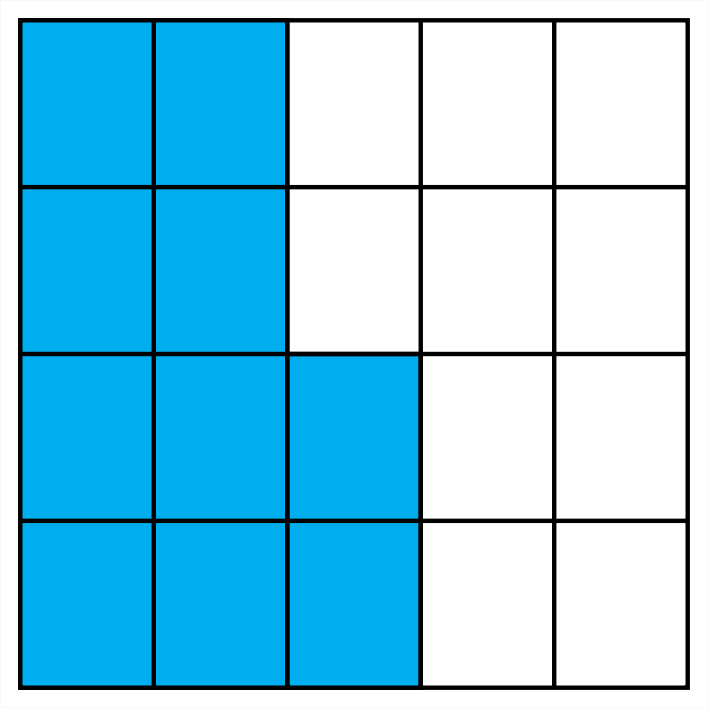
\includegraphics[width=48px]{../images/imagen_frac01.png} \fillin[\fbox{$\dfrac{10}{20}$}][0in]   \\[2em]
				\part 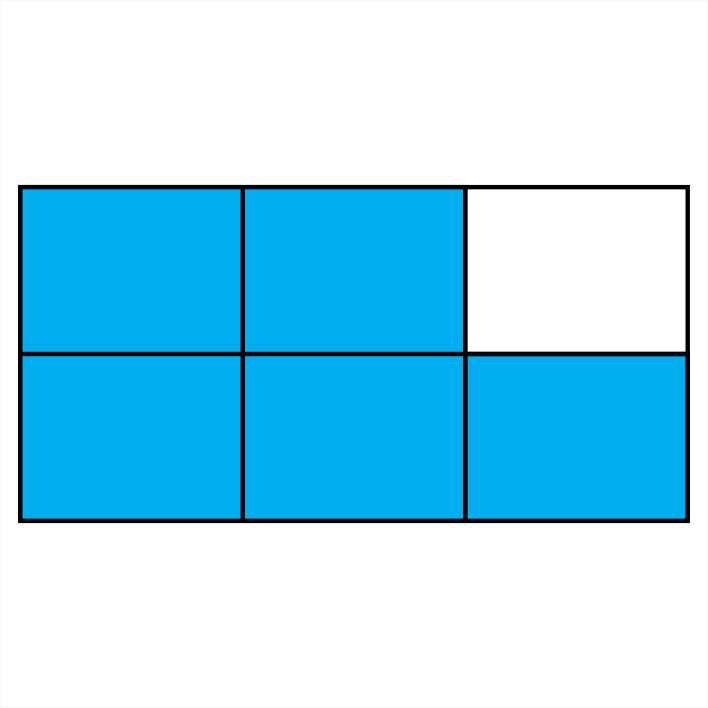
\includegraphics[width=48px]{../images/imagen_frac02.png} \fillin[\fbox{$\dfrac{5}{6}$}][0in]     \\[2em]
				% \part 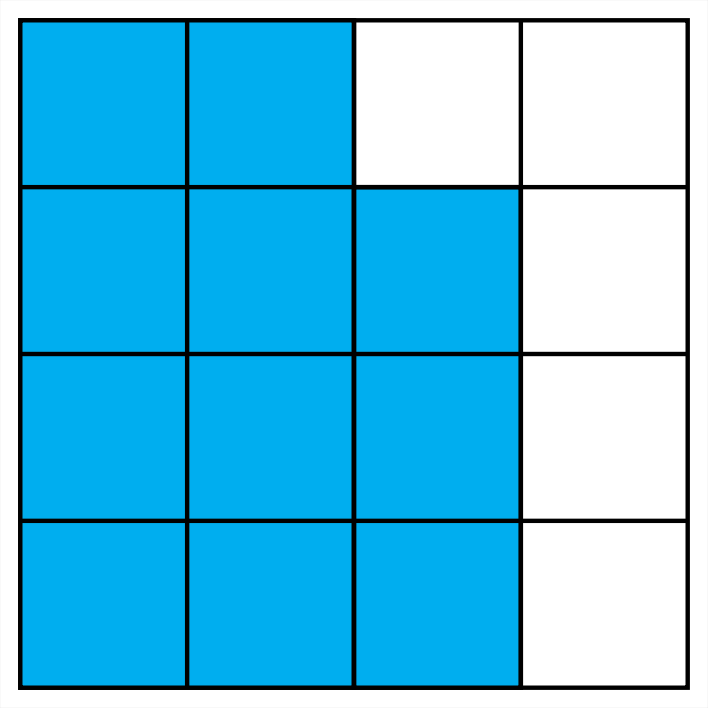
\includegraphics[width=48px]{../images/imagen_frac03.png} \fillin[\fbox{$\dfrac{11}{16}$}][0in]   \\[2em]
				% \part 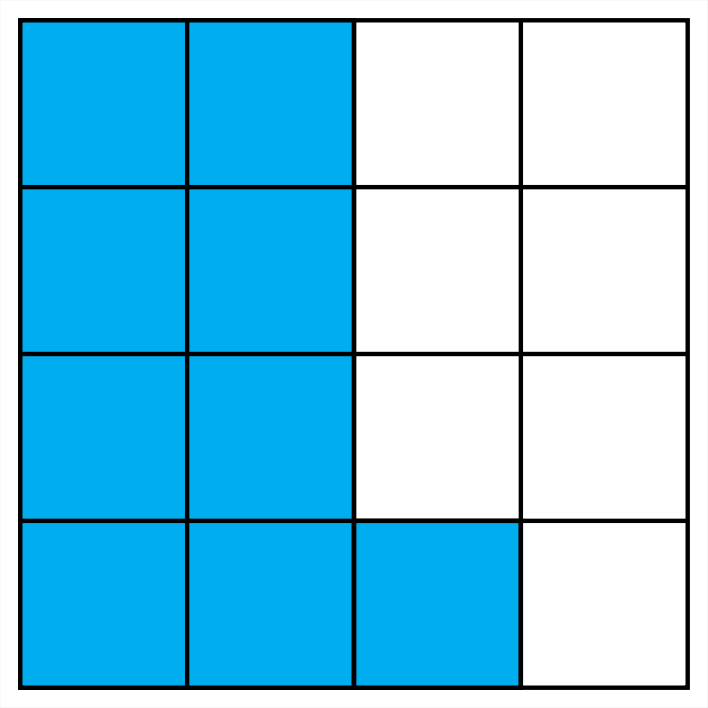
\includegraphics[width=48px]{../images/imagen_frac06.png} \fillin[\fbox{$\dfrac{9}{16}$}][0in]    \\[2em]
				% \part 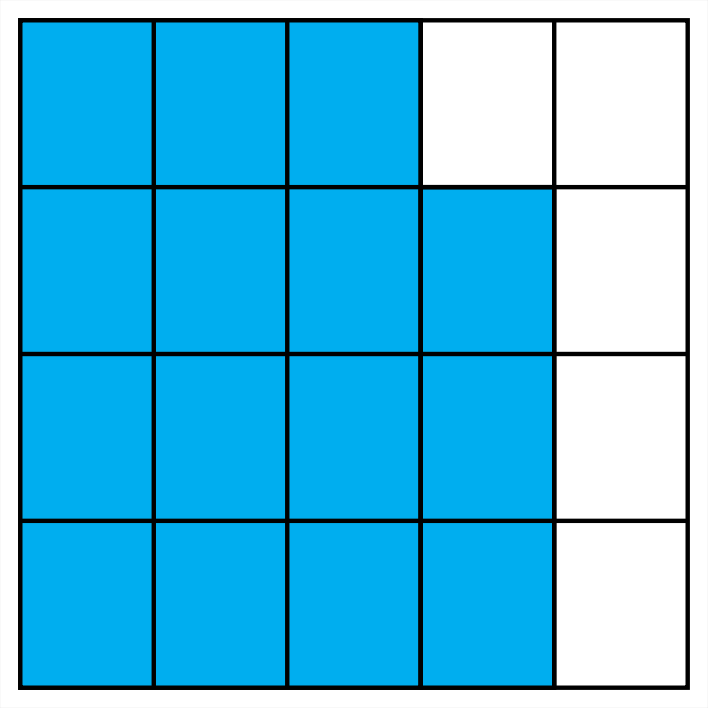
\includegraphics[width=48px]{../images/imagen_frac07.png} \fillin[\fbox{$\dfrac{15}{20}$}][0in]   \\[2em]
				% \part 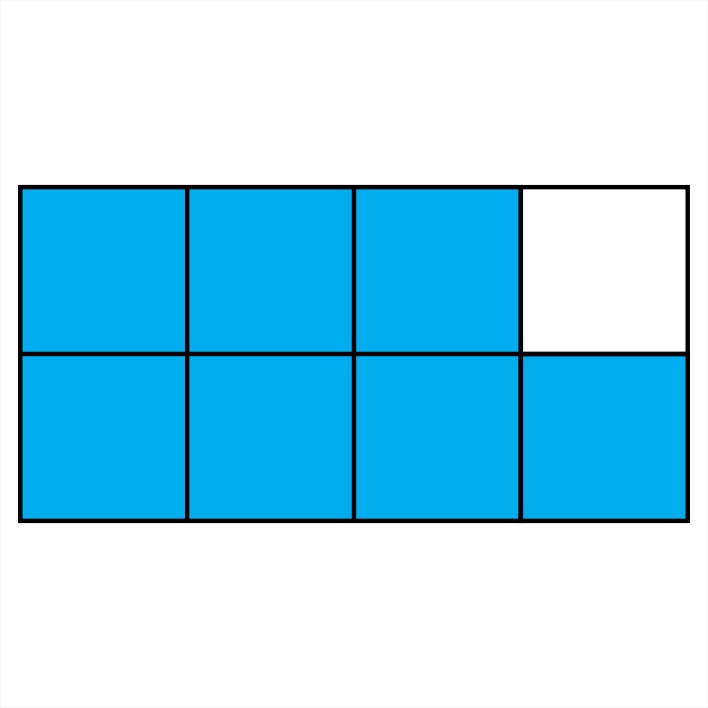
\includegraphics[width=48px]{../images/imagen_frac08.png} \fillin[\fbox{$\dfrac{7}{8}$}][0in]     \\[2em]
				\part 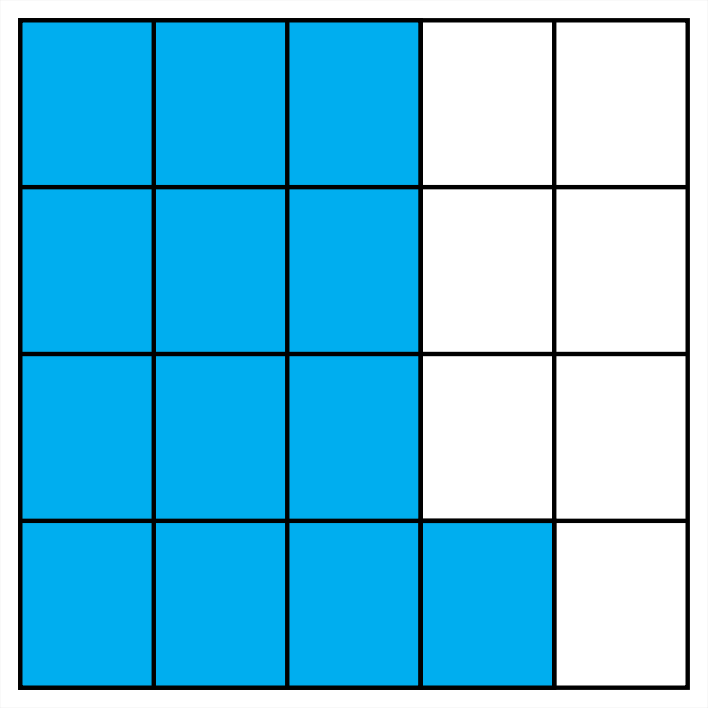
\includegraphics[width=48px]{../images/imagen_frac09.png} \fillin[\fbox{$\dfrac{13}{20}$}][0in]   \\[2em]
				\part 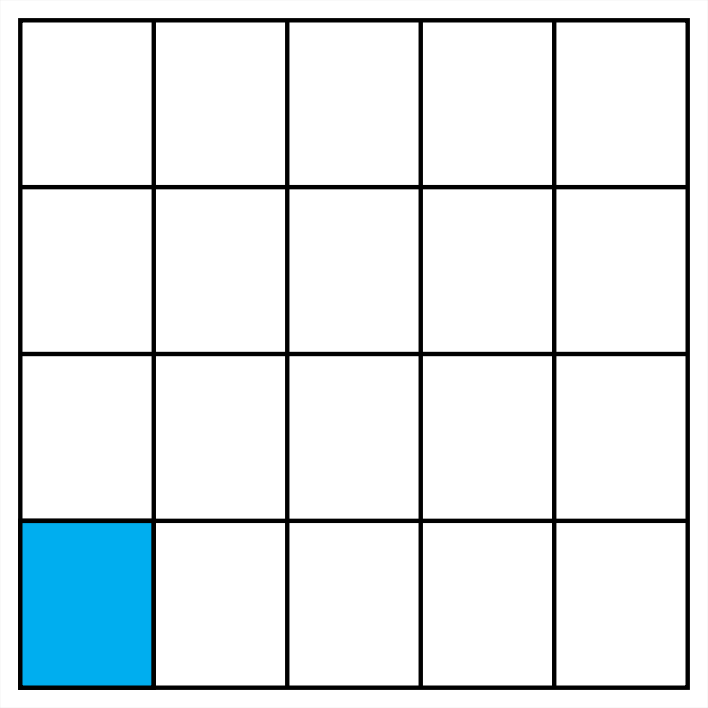
\includegraphics[width=48px]{../images/imagen_frac11.png} \fillin[\fbox{$\dfrac{1}{20}$}][0in]    \\[2em]
			\end{parts}
		\end{multicols}
	}


      \questionboxed[4]{Escribe sobre la línea la fracción que representa cada imagen:
      
      \begin{multicols}{3}
                  \begin{parts}
                        \part 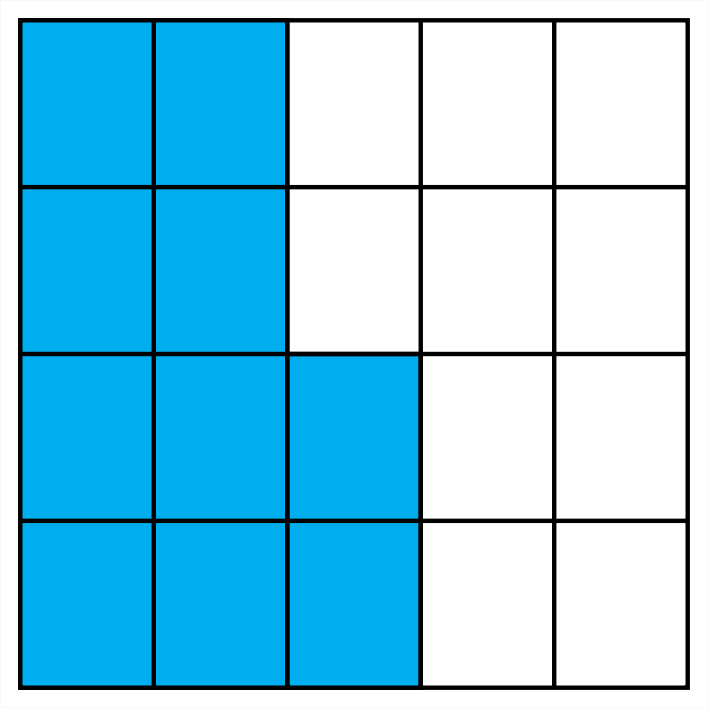
\includegraphics[width=50px]{../images/imagen_frac01.png} \fillin[$\dfrac{10}{20}$][1in]
                        \part 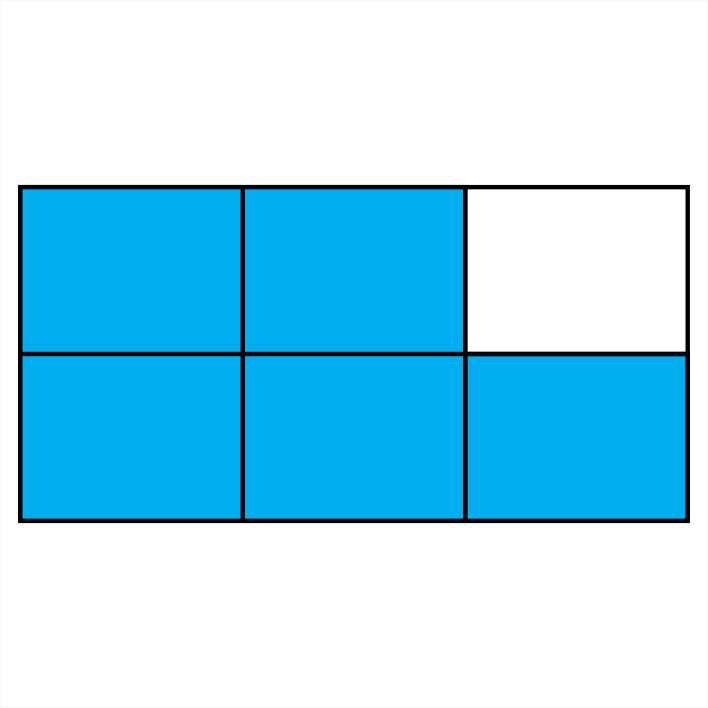
\includegraphics[width=50px]{../images/imagen_frac02.png} \fillin[$\dfrac{5}{6}$][1in]
                        \part 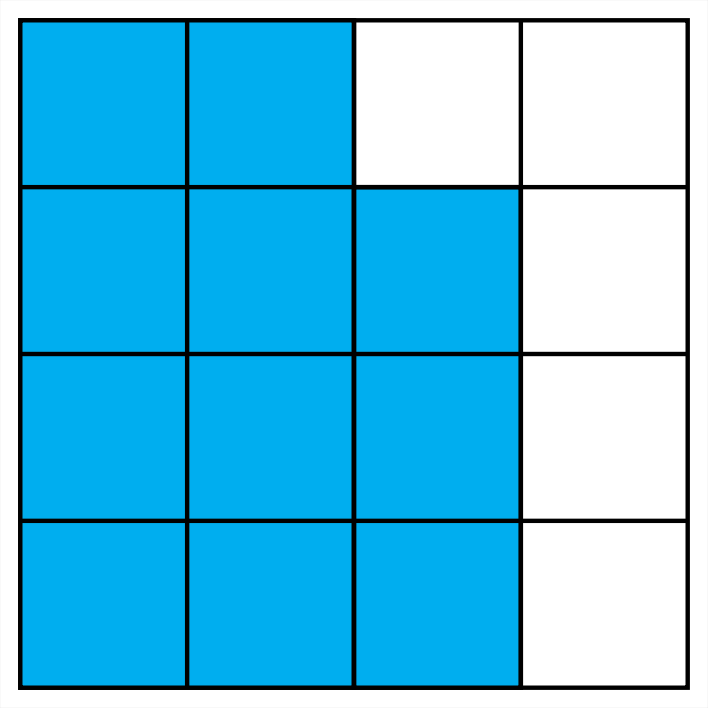
\includegraphics[width=50px]{../images/imagen_frac03.png} \fillin[$\dfrac{11}{16}$][1in]
                        \part 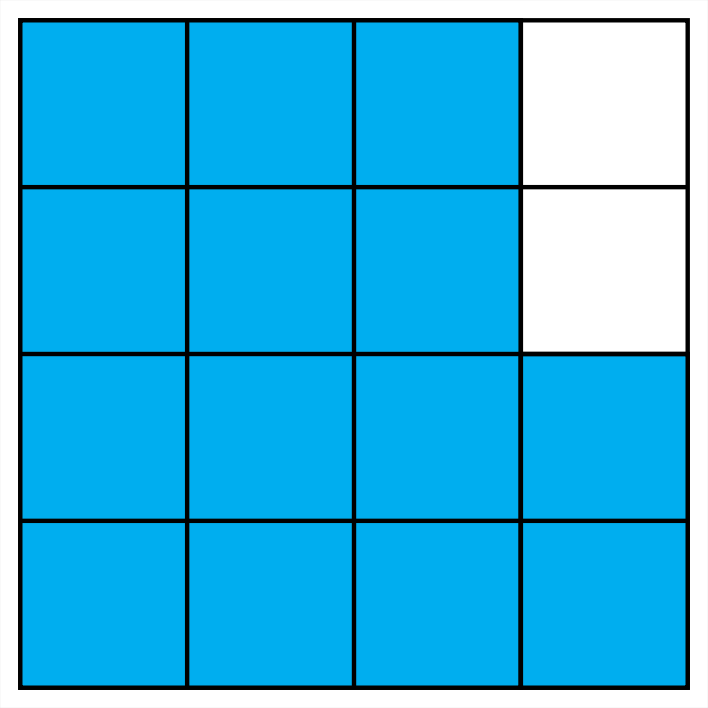
\includegraphics[width=50px]{../images/imagen_frac04.png} \fillin[$\dfrac{14}{16}$][1in]
                        % \part 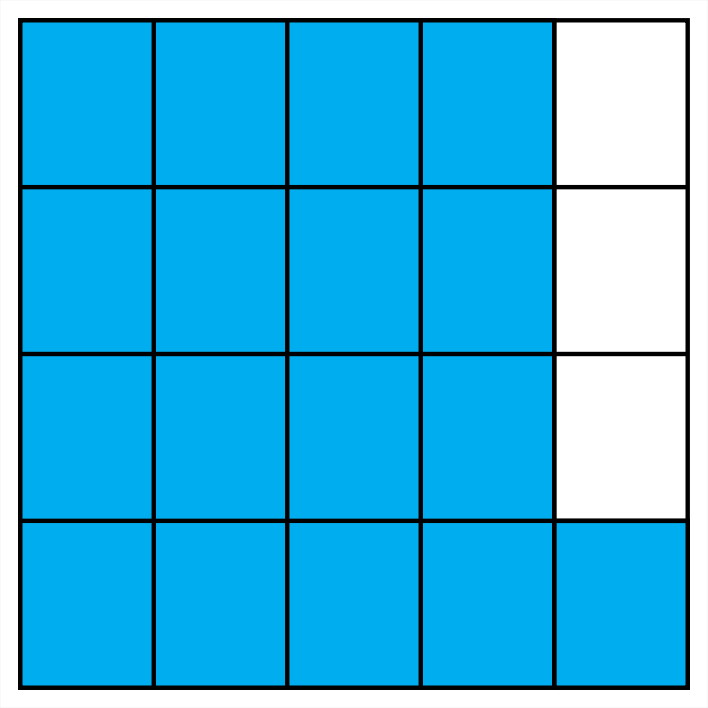
\includegraphics[width=100px]{../images/imagen_frac05.png} \fillin[$\dfrac{10}{20}$][1in]
                        % \part 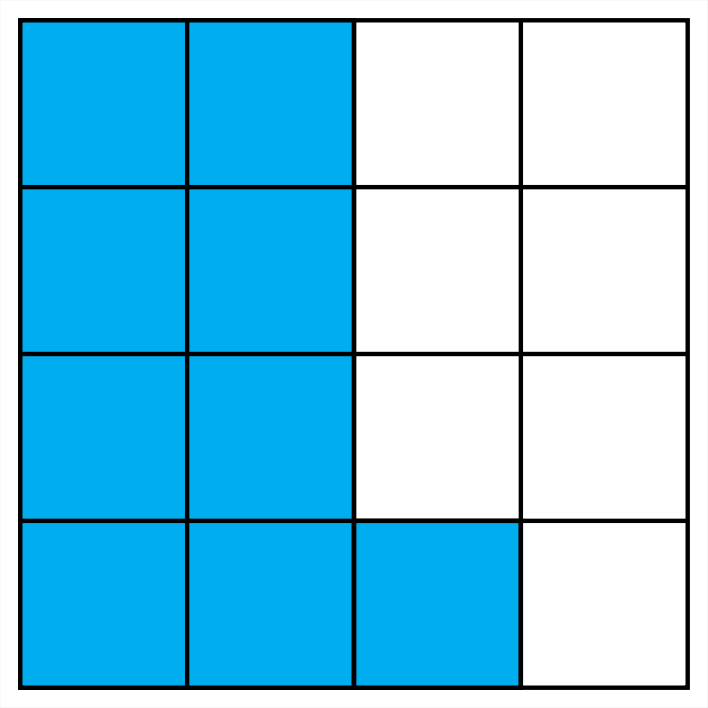
\includegraphics[width=100px]{../images/imagen_frac06.png} \fillin[$\dfrac{10}{20}$][1in]
                        \part 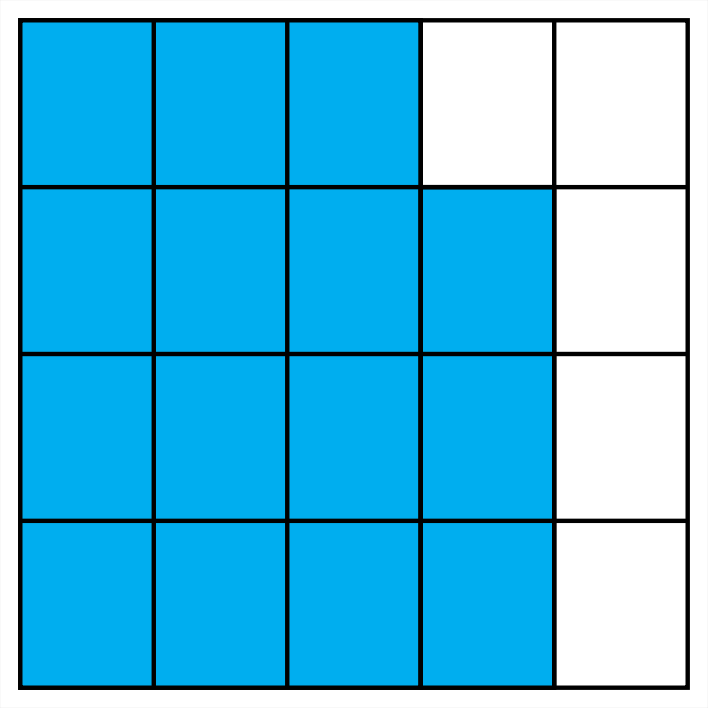
\includegraphics[width=50px]{../images/imagen_frac07.png} \fillin[$\dfrac{15}{20}$][1in]
                        \part 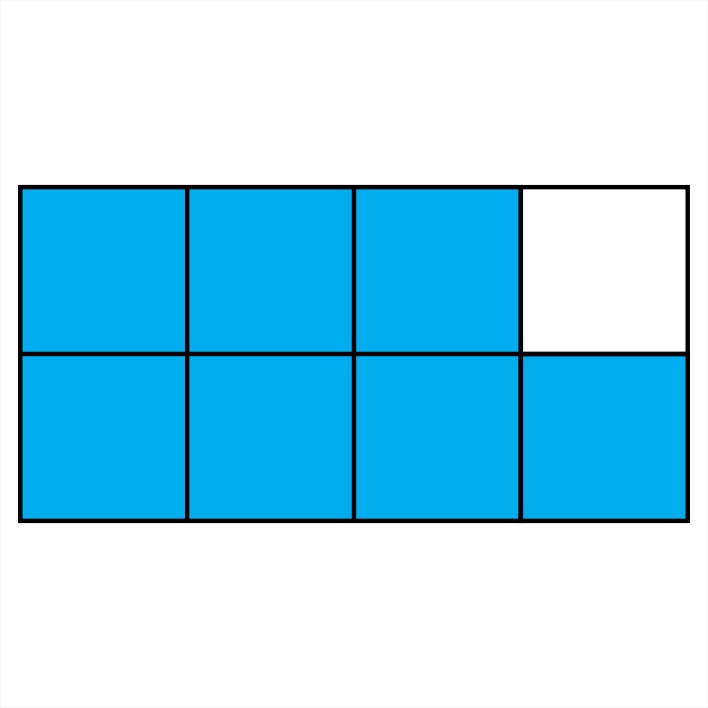
\includegraphics[width=50px]{../images/imagen_frac08.png} \fillin[$\dfrac{7}{8}$][1in]
                        % \part 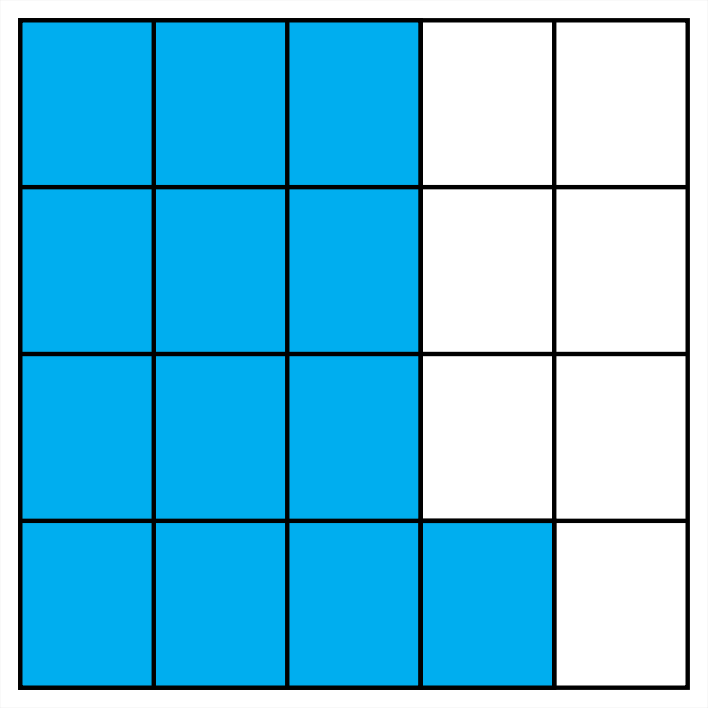
\includegraphics[width=100px]{../images/imagen_frac09.png} \fillin[$\dfrac{10}{20}$][1in]
                        % \part 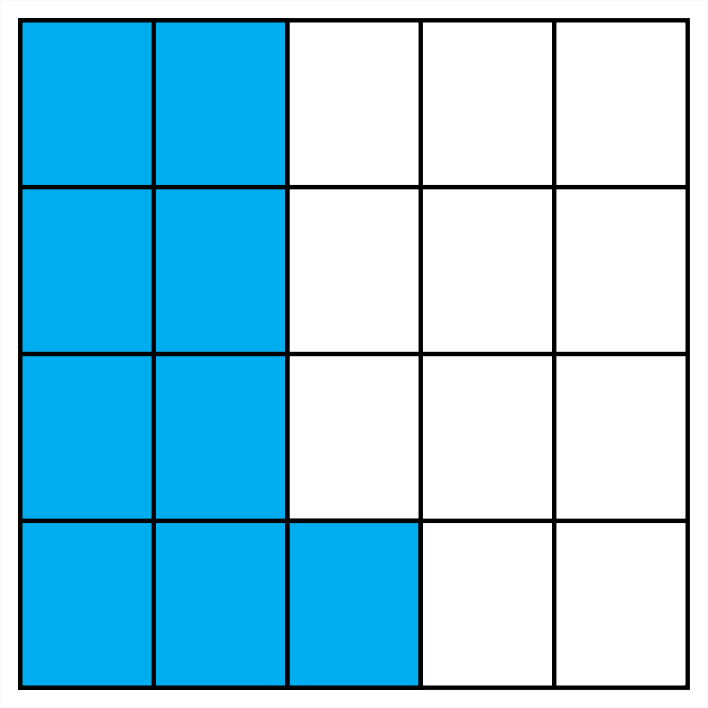
\includegraphics[width=100px]{../images/imagen_frac10.png} \fillin[$\dfrac{10}{20}$][1in]
                  \end{parts}
            \end{multicols}
      }

      \subsection{Fracciones, M.C.M. y M.C.D.}
      
      \subsubsection{Conversión de fracciones}

	  \ejemplosboxed[4]{Convierte la siguientes fracciones impropias a mixtas:

	\begin{multicols}{3}
		\begin{parts}
			\part $\dfrac{13}{3}= $ \fillin[$4\dfrac{1}{3}$][0in]
			% \part $\dfrac{63}{10}= $ \fillin[$6\dfrac{3}{10}$][0in]
			\part $\dfrac{51}{5}= $ \fillin[$10\dfrac{1}{5}$][0in]
		\end{parts}
	\end{multicols}
	}

      \questionboxed[4]{Convierte la siguientes fracciones impropias a mixtas:
            
      \begin{multicols}{3}
                  \begin{parts}
                        \part $\dfrac{23}{3}= $ \fillin[$7\dfrac{2}{3}$][0in]
                        \part $\dfrac{63}{10}= $ \fillin[$6\dfrac{3}{10}$][0in]
						\part $\dfrac{38}{6}= $ \fillin[$6\dfrac{2}{6}$][0in]
                  \end{parts}
            \end{multicols}
      }

      \subsubsection{Nombre de fracciones}

	  \ejemplosboxed[4]{Escribe la fracción que corresponda en cada inciso:

	\begin{parts}
		% \part ¿Cómo se escribe numéricamente la fracción \textbf{ocho quintos}?    \fillin[$\dfrac{8}{5}$][0in]  \\
		\part ¿Cómo se escribe numéricamente la fracción \textbf{seis onceavos}?   \fillin[$\dfrac{6}{11}$][0in] \\
		% \part ¿Cómo se escribe numéricamente la fracción \textbf{dos séptimos}?    \fillin[$\dfrac{2}{7}$][0in]  \\
		\part ¿Cómo se escribe numéricamente la fracción \textbf{once medios}?     \fillin[$\dfrac{11}{2}$][0in] \\
		% \part ¿Cómo se escribe numéricamente la fracción \textbf{diez décimos}?    \fillin[$\dfrac{10}{10}$][0in]\\
	\end{parts}
	  }

      \questionboxed[4]{Escribe la fracción que corresponda en cada inciso:
           
      \begin{parts}
                  \part ¿Cómo se escribe numéricamente la fracción \textbf{ocho quintos}?    \fillin[$\dfrac{8}{5}$][0in]  
                 
				  \part ¿Cómo se escribe numéricamente la fracción \textbf{seis onceavos}?   \fillin[$\dfrac{6}{11}$][0in] 
                 
				  \part ¿Cómo se escribe numéricamente la fracción \textbf{dos séptimos}?    \fillin[$\dfrac{2}{7}$][0in]  
                 
				  \part ¿Cómo se escribe numéricamente la fracción \textbf{once medios}?     \fillin[$\dfrac{11}{2}$][0in] 
                 
				  \part ¿Cómo se escribe numéricamente la fracción \textbf{diez décimos}?    \fillin[$\dfrac{10}{10}$][0in]
            \end{parts}
      }

      \subsubsection{Fracciones en la recta numérica}

	  	\ejemplosboxed[4]{Escribe la fracción que representa el punto en la recta numérica

	\begin{multicols}{2}
		\begin{parts}
			\part 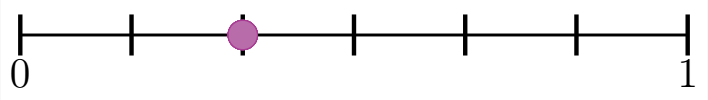
\includegraphics[width=150px]{../images/recta_num_frac01.png} \\[-0.5em] \fillin[$\dfrac{2}{6}$][2in]
			\part 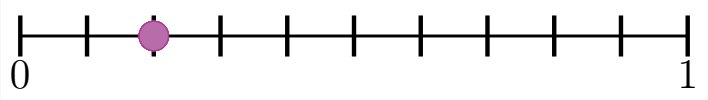
\includegraphics[width=150px]{../images/recta_num_frac02.png} \\[-0.5em] \fillin[$\dfrac{2}{10}$][2in]
			% \part 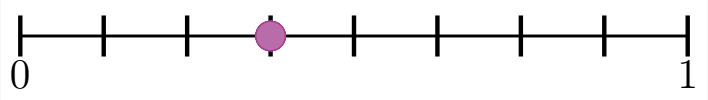
\includegraphics[width=150px]{../images/recta_num_frac03.png} \\[-0.5em] \fillin[$\dfrac{2}{6}$][1.5in]
			% \part 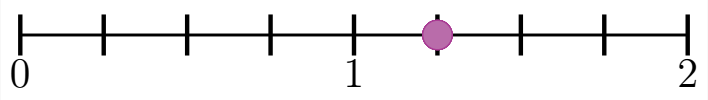
\includegraphics[width=150px]{../images/recta_num_frac04.png} \\[-0.5em] \fillin[$\dfrac{2}{6}$][1.5in]
			% \part 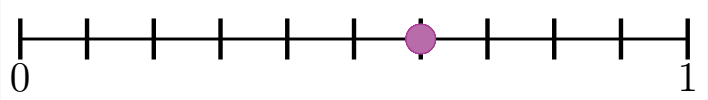
\includegraphics[width=150px]{../images/recta_num_frac05.png} \\[-0.5em] \fillin[$\dfrac{2}{6}$][1.5in]
			% \part 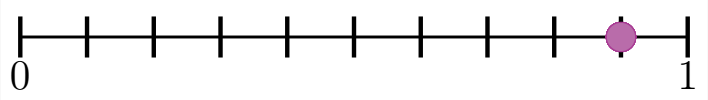
\includegraphics[width=150px]{../images/recta_num_frac06.png} \\[-0.5em] \fillin[$\dfrac{2}{6}$][1.5in]
			% \part 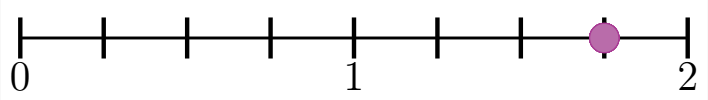
\includegraphics[width=150px]{../images/recta_num_frac07.png} \\[-0.5em] \fillin[$\dfrac{2}{6}$][1.5in]
			% \part 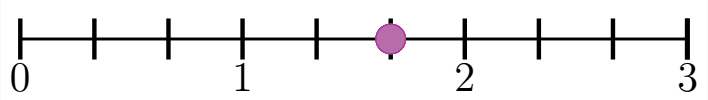
\includegraphics[width=150px]{../images/recta_num_frac08.png} \\[-0.5em] \fillin[$\dfrac{2}{6}$][1.5in]
			% \part 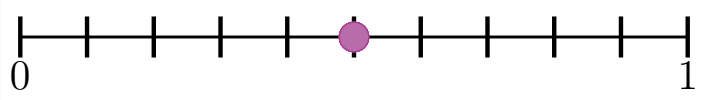
\includegraphics[width=150px]{../images/recta_num_frac09.png} \\[-0.5em] \fillin[$\dfrac{2}{6}$][1.5in]
			% \part 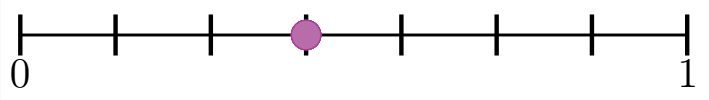
\includegraphics[width=150px]{../images/recta_num_frac10.png} \\[-0.5em] \fillin[$\dfrac{2}{6}$][1.5in]
		\end{parts}
	\end{multicols}
	}

      \questionboxed[4]{Escribe la fracción que representa el punto en la recta numérica
           
      \begin{multicols}{3}
                  \begin{parts}
                        \part 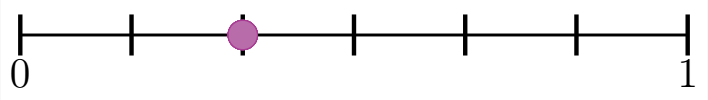
\includegraphics[width=\linewidth]{../images/recta_num_frac01.png} \\ \fillin[$\dfrac{2}{6}$][1in]
                        
						\part 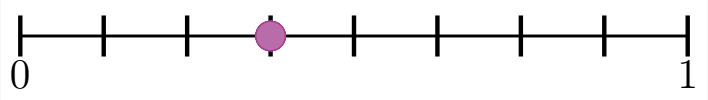
\includegraphics[width=\linewidth]{../images/recta_num_frac03.png} \\ \fillin[$\dfrac{3}{8}$][1in]
                        
						\part 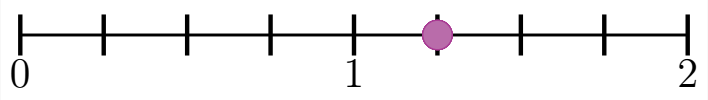
\includegraphics[width=\linewidth]{../images/recta_num_frac04.png} \\ \fillin[$\dfrac{5}{4}$][1in]
                        
						\part 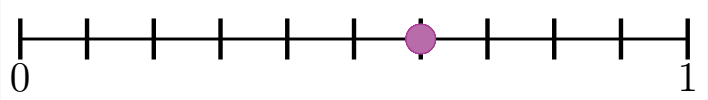
\includegraphics[width=\linewidth]{../images/recta_num_frac05.png} \\ \fillin[$\dfrac{6}{10}$][1in]
                        
						\part 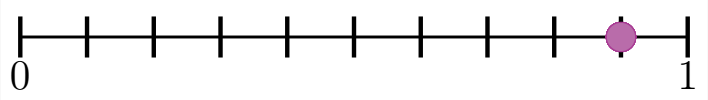
\includegraphics[width=\linewidth]{../images/recta_num_frac06.png} \\ \fillin[$\dfrac{9}{10}$][1in]
                        
						\part 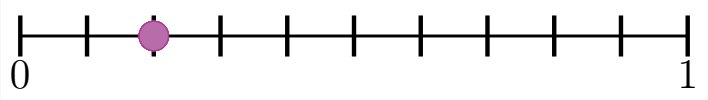
\includegraphics[width=\linewidth]{../images/recta_num_frac02.png} \\ \fillin[$\dfrac{2}{10}$][1in]
                        
						\part 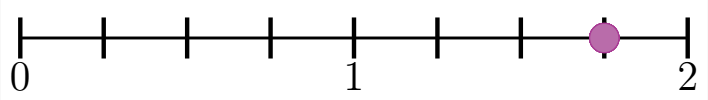
\includegraphics[width=\linewidth]{../images/recta_num_frac07.png} \\ \fillin[$\dfrac{7}{4}$][1in]
                        
						\part 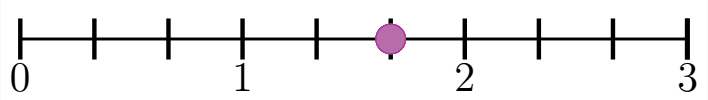
\includegraphics[width=\linewidth]{../images/recta_num_frac08.png} \\ \fillin[$\dfrac{5}{3}$][1in]
                        
						\part 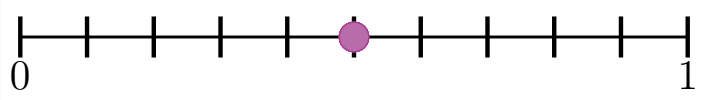
\includegraphics[width=\linewidth]{../images/recta_num_frac09.png} \\ \fillin[$\dfrac{5}{10}$][1in]
                        % \part 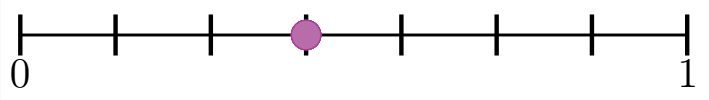
\includegraphics[width=\linewidth]{../images/recta_num_frac10.png} \\ \fillin[$\dfrac{3}{7}$][1in]
                  \end{parts}
            \end{multicols}
      }

      \subsubsection{Simplificación de fracciones}

	  	\ejemplosboxed[4]{Simplifica a su mínima expresión la siguiente fracción usando el máximo común divisor

	\begin{multicols}{2}
		\begin{parts}
			\part $\dfrac{8}{64}=$ \fillin[$\dfrac{1}{8}$][0in]
			\part $\dfrac{6}{42}=$ \fillin[$\dfrac{1}{7}$][0in]
		\end{parts}
	\end{multicols}
	}

	\questionboxed[4]{Simplifica a su mínima expresión la siguiente fracción usando el máximo común divisor
      
      \begin{multicols}{3}
                  \begin{parts}
                        \part $\dfrac{6}{42}=$ \fillin[$\dfrac{1}{7}$][0in]\\[1em]
						
                        \part $\dfrac{12}{18}=$ \fillin[$\dfrac{2}{3}$][0in]\\[1em]
						
                        \part $\dfrac{15}{30}=$ \fillin[$\dfrac{1}{2}$][0in]\\[1em]
						
                        \part $\dfrac{24}{36}=$ \fillin[$\dfrac{2}{3}$][0in]\\[1em]
						
                        \part $\dfrac{8}{64}=$ \fillin[$\dfrac{1}{8}$][0in]\\[1em]
						
                        \part $\dfrac{16}{24}=$ \fillin[$\dfrac{2}{3}$][0in]\\[1em]
						
                  \end{parts}
            \end{multicols}
      }

  \subsubsection{Fracciones equivalentes}
  
  \ejemplosboxed[4]{Indica si las siguientes fracciones son equivalentes o no:

	\begin{multicols}{2}
		\begin{parts}
			\part $\dfrac{2}{5}=\dfrac{8}{10}$\qquad
			\begin{oneparcheckboxes}
				\choice Sí
				\CorrectChoice No
			\end{oneparcheckboxes}

			\part $\dfrac{2}{8}=\dfrac{4}{16}$\qquad
			\begin{oneparcheckboxes}
				\CorrectChoice Sí
				\choice No
			\end{oneparcheckboxes}

			\part $\dfrac{1}{5}=\dfrac{5}{1}$\qquad
			\begin{oneparcheckboxes}
				\choice Sí
				\CorrectChoice No
			\end{oneparcheckboxes}

			\part $\dfrac{1}{10}=\dfrac{3}{30}$\qquad
			\begin{oneparcheckboxes}
				\CorrectChoice Sí
				\choice No
			\end{oneparcheckboxes}
		\end{parts}
	\end{multicols}
  }


  \questionboxed[2]{Indica si las siguientes fracciones son equivalentes o no:
  
  \begin{multicols}{2}
                  \begin{parts}
                        \part $\dfrac{4}{5}=\dfrac{8}{10}$\qquad
                        \begin{oneparcheckboxes}
                              \CorrectChoice Sí
                              \choice No
                        \end{oneparcheckboxes}

                        \part $\dfrac{1}{8}=\dfrac{4}{16}$\qquad
                        \begin{oneparcheckboxes}
                              \choice Sí
                              \CorrectChoice No
                        \end{oneparcheckboxes}

                        \part $\dfrac{1}{5}=\dfrac{5}{10}$\qquad
                        \begin{oneparcheckboxes}
                              \choice Sí
                              \CorrectChoice No
                        \end{oneparcheckboxes}

                        \part $\dfrac{1}{10}=\dfrac{3}{30}$\qquad
                        \begin{oneparcheckboxes}
                              \CorrectChoice Sí
                              \choice No
                        \end{oneparcheckboxes}

                        \part $\dfrac{1}{4}=\dfrac{2}{4}$\qquad
                        \begin{oneparcheckboxes}
                              \choice Sí
                              \CorrectChoice No
                        \end{oneparcheckboxes}

                        \part $\dfrac{3}{2}=\dfrac{12}{8}$\qquad
                        \begin{oneparcheckboxes}
                              \CorrectChoice Sí
                              \choice No
                        \end{oneparcheckboxes}

                        \part $\dfrac{3}{6}=\dfrac{1}{3}$\qquad
                        \begin{oneparcheckboxes}
                              \choice Sí
                              \CorrectChoice No
                        \end{oneparcheckboxes}

                        \part $\dfrac{18}{12}=\dfrac{9}{4}$\qquad
                        \begin{oneparcheckboxes}
                              \choice Sí
                              \CorrectChoice No
                        \end{oneparcheckboxes}
                  \end{parts}
            \end{multicols}
      }

      \subsubsection{Comparación de fracciones}
     
	  	\ejemplosboxed[4]{Compara las siguientes fracciones usando los signos mayor que (>), menor que (<) o igual (=):

	\begin{multicols}{4}
		\begin{parts}
			\part $\dfrac{4}{3}$ \fillin[$>$][0.5in] $\dfrac{5}{4}$\\[0.75em]
			\part $\dfrac{1}{3}$ \fillin[$=$][0.5in] $\dfrac{3}{9}$\\[0.75em]
			% \part $\dfrac{2}{3}$ \fillin[$<$][0.5in] $\dfrac{3}{2}$\\[0.75em]
			% \part $\dfrac{3}{4}$ \fillin[$>$][0.5in] $\dfrac{2}{3}$\\[0.75em]
			\part $\dfrac{5}{6}$ \fillin[$>$][0.5in] $\dfrac{4}{5}$\\[0.75em]
			\part $\dfrac{1}{3}$ \fillin[$<$][0.5in] $\dfrac{2}{5}$\\[0.75em]
		\end{parts}
	\end{multicols}
	}

      \questionboxed[4]{Compara las siguientes fracciones usando los signos mayor que (>), menor que (<) o igual (=):
         
      \begin{multicols}{3}
                  \begin{parts}
                        % \part $\dfrac{2}{5}$ \fillin[$>$][0.5in] $\dfrac{1}{3}$\\[0.25em]
                        \part $\dfrac{3}{4}$ \fillin[$<$][0.5in] $\dfrac{4}{5}$\\[0.25em]
                        
						\part $\dfrac{2}{5}$ \fillin[$<$][0.5in] $\dfrac{2}{3}$\\[0.25em]
                        
						\part $\dfrac{1}{5}$ \fillin[$<$][0.5in] $\dfrac{1}{4}$\\[0.25em]
                        
						\part $\dfrac{3}{2}$ \fillin[$=$][0.5in] $\dfrac{9}{6}$\\[0.25em]
                        
						\part $\dfrac{5}{6}$ \fillin[$>$][0.5in] $\dfrac{4}{6}$\\[0.25em]
                        
						\part $\dfrac{4}{3}$ \fillin[$>$][0.5in] $\dfrac{5}{4}$\\[0.25em]
                        
						\part $\dfrac{1}{3}$ \fillin[$=$][0.5in] $\dfrac{9}{3}$\\[0.25em]
                        
						\part $\dfrac{2}{3}$ \fillin[$<$][0.5in] $\dfrac{3}{2}$\\[0.25em]
                        % \part $\dfrac{3}{5}$ \fillin[$>$][0.5in] $\dfrac{2}{3}$\\[0.25em]
                        
						\part $\dfrac{5}{6}$ \fillin[$>$][0.5in] $\dfrac{4}{5}$\\[0.25em]
                  \end{parts}
            \end{multicols}
      }

      \subsubsection{M.C.D y M.C.M}
   
	  \ejemplosboxed[4]{Calcula lo que se te pide en cada inciso:

	\begin{multicols}{2}
		\begin{parts}
			\part Encuentra el máximo común divisor de 120 y 300.

			\begin{solutionbox}{1cm}
				Se calcula el MCD$(120,300) = 60$.
			\end{solutionbox}

\columnbreak%

			\part Encuentra el mínimo común múltiplo de 12, 15 y 18.

			\begin{solutionbox}{1cm}
				Se calcula el MCM$(12,15,18) = 180$.
			\end{solutionbox}

		\end{parts}
	\end{multicols}
	}

      \questionboxed[4]{Calcula lo que se te pide en cada inciso:
    
      \begin{multicols}{2}
            \begin{parts}
                  \part Encuentra el mínimo común múltiplo de 2 y 9.
              
                  \begin{solutionbox}{2cm}
                        El mínimo común múltiplo de 2 y 9 es 18.
                  \end{solutionbox}

                  \part Encuentra el máximo común divisor de 5 y 15.
            
                  \begin{solutionbox}{2cm}
                        El máximo común divisor de 5 y 15 es 5.
                  \end{solutionbox}

                  % \part Encuentra el mínimo común múltiplo de 2 y 5.
   
                  % \begin{solutionbox}{1.2cm}
                  %       El mínimo común múltiplo de 2 y 5 es 10.
                  % \end{solutionbox}

                  \part Encuentra el máximo común divisor de 33 y 121.
            
                  \begin{solutionbox}{2cm}
                        El máximo común divisor de 33 y 121 es 11.
                  \end{solutionbox}

                  \part Encuentra el máximo común divisor de 25 y 100.
             
                  \begin{solutionbox}{2cm}
                        El máximo común divisor de 25 y 100 es 25.
                  \end{solutionbox}

                  \part Encuentra el máximo común divisor de 18 y 36.
              
                  \begin{solutionbox}{2cm}
                        El máximo común divisor de 18 y 36 es 18.
                  \end{solutionbox}

                  % \part Encuentra el mínimo común múltiplo de 4 y 9.
               
                  % \begin{solutionbox}{1.2cm}
                  %       El mínimo común múltiplo de 4 y 9 es 36.
                  % \end{solutionbox}

                  % \part Encuentra el mínimo común múltiplo de 6 y 7.
                
                  % \begin{solutionbox}{1.2cm}
                  %       El mínimo común múltiplo de 6 y 7 es 42.
                  % \end{solutionbox}

                  \part Encuentra el mínimo común múltiplo de 2, 3 y 4.
                 
                  \begin{solutionbox}{1.2cm}
                        El mínimo común múltiplo de 2, 3 y 4 es 12.
                  \end{solutionbox}

                  \part Encuentra el máximo común divisor de 2 y 14.
                  
                  \begin{solutionbox}{1.2cm}
                        El máximo común divisor de 2 y 14 es 2.
                  \end{solutionbox}
            
                  \part Encuentra el mínimo común múltiplo de 12, 15 y 18.
                 
                  \begin{solutionbox}{1.2cm}
                        El mínimo común múltiplo de 12, 15 y 18 es 180.
                  \end{solutionbox}
            \end{parts}
      \end{multicols}
      }

      \subsubsection{Resolución de problemas}

	    \ejemplosboxed[2]{María y Jorge tienen 24 bolas blancas, 40 bolas azules y 72 bolas rojas y quieren hacer el mayor número de collares iguales sin que sobre ninguna bola. ¿Cuántos collares iguales pueden hacer?
         
      \begin{solutionbox}{2cm}
                  Se calcula el M.C.D.$(24,40,72) = 8$.\\
                  Por lo tanto, se pueden hacer 8 collares.
            \end{solutionbox}
      }

      \questionboxed[3]{María y Jorge tienen 45 bolas blancas, 15 bolas azules y 90 bolas rojas y quieren hacer el mayor número de collares iguales sin que sobre ninguna bola. ¿Cuántos collares iguales pueden hacer?
         
      \begin{solutionbox}{2cm}
                  Se calcula el M.C.D.$(45,15,90) = 15$.\\
                  Por lo tanto, se pueden hacer 15 collares.
            \end{solutionbox}
      }

	\subsection{Operaciones con fracciones}
	
\ejemplosboxed[6]{Realiza las siguientes operaciones con fracciones (simplifica el resultado a la mínima expresión):

    \begin{multicols}{3}

        \begin{parts}\large
				\subsubsection{Suma y resta con denominadores iguales}

            \part $\dfrac{7}{8}-\dfrac{3}{8}=$ \fillin[$\dfrac{4}{8}=\dfrac{1}{2}$][0in]\\[0.5em]
	
			\subsubsection{Multiplicación de fracciones}

            \part $\dfrac{9}{5}\times\dfrac{15}{4}=$ \fillin[$\dfrac{135}{20}=\dfrac{27}{4}$][0in]\\[0.5em]
          
			\columnbreak%

				\subsubsection{Suma y resta denominadores diferentes}

            \part $\dfrac{7}{8}-\dfrac{3}{7}=$ \fillin[$\dfrac{49}{56}-\dfrac{24}{56}=\dfrac{25}{56}$][0in] \\[3em]

            \part $\dfrac{5}{8}+\dfrac{3}{4}=$ \fillin[$\dfrac{5}{8}+\dfrac{6}{8}=\dfrac{11}{8}$][0in]  \\[3em]
              	
			\columnbreak%

			\subsubsection{División de fracciones}
			
            \part $\dfrac{3}{5} \divisionsymbol\dfrac{2}{3}=$ \fillin[$\dfrac{9}{10}$][0in]  \\[1em]

            \part $\dfrac{7}{12}\divisionsymbol\dfrac{2}{3}=$ \fillin[$\dfrac{21}{24}=\dfrac{7}{8}$][0in]\\[1em]

        \end{parts}
    \end{multicols}
	}

	% \subsubsection{Suma y resta con denominadores iguales}

	\questionboxed[3]{ Realiza las siguientes sumas y restas de fracciones con denominadores iguales:
		\begin{multicols}{3}
			\begin{parts}\LARGE
				\part $\dfrac{3}{5}+\dfrac{2}{5}=$ \fillin[$\dfrac{5}{5}=1$][0in]\\[1em]
				\part $\dfrac{7}{8}-\dfrac{3}{8}=$ \fillin[$\dfrac{5}{8}$][0in]\\[1em]
				\part $\dfrac{37}{12}-\dfrac{11}{12}=$ \fillin[$\dfrac{13}{6}=1$][0in]\\[1em]
				% \part $\dfrac{7}{4}+\dfrac{3}{4}=$ \fillin[$\dfrac{}{}+\dfrac{}{}=\dfrac{}{}$][0in]\\[1em]
				% \part $\dfrac{1}{3}+\dfrac{2}{3}=$ \fillin[$\dfrac{}{}+\dfrac{}{}=\dfrac{}{}$][0in]\\[1em]
				% \part $\dfrac{5}{4}+\dfrac{8}{4}=$ \fillin[$\dfrac{}{}+\dfrac{}{}=\dfrac{}{}$][0in]\\[1em]
			\end{parts}
		\end{multicols}
	}

	% \subsubsection{Suma y resta denominadores diferentes}
	\questionboxed[5]{ Realiza las siguientes sumas y restas de fracciones con denominadores diferentes:
		\begin{multicols}{3}
			\begin{parts}\large
				\part $\dfrac{3}{5}+\dfrac{2}{3}=$ \fillin[$\dfrac{9}{15}+\dfrac{10}{15}=\dfrac{19}{15}$][0in]\\[1em]
				\part $\dfrac{7}{8}+\dfrac{3}{4}=$ \fillin[$\dfrac{7}{8}+\dfrac{6}{8}=\dfrac{13}{8}$][0in]\\[1em]
				\part $\dfrac{2}{3}-\dfrac{1}{6}=$ \fillin[$\dfrac{2}{3}-\dfrac{1}{6} =\dfrac{1}{2}$][0in]\\[1em]
				\part $\dfrac{5}{6}-\dfrac{3}{8}=$ \fillin[$\dfrac{5}{6}-\dfrac{3}{8} =\dfrac{11}{24}$][0in]\\[1em]
				\part $\dfrac{4}{5}-\dfrac{3}{10}=$ \fillin[$\dfrac{4}{5}-\dfrac{3}{10} =\dfrac{1}{2}$][0in]\\[1em]
				\part $\dfrac{1}{3}-\dfrac{1}{5}=$ \fillin[$\dfrac{1}{3}-\dfrac{1}{5} = \dfrac{2}{5}$][0in]\\[1em]
			\end{parts}
		\end{multicols}
	}

	% \subsubsection{Multiplicación de fracciones}
	\questionboxed[6]{ Realiza las siguientes multiplicaciones de fracciones:
		
	\begin{multicols}{3}
			\begin{parts}\large
				\part $\dfrac{3}{5}\times\dfrac{2}{3}=$ \fillin[$\dfrac{6}{15}$][0in]\\[1em]
				\part $\dfrac{7}{8}\times\dfrac{3}{4}=$ \fillin[$\dfrac{21}{32}$][0in]\\[1em]
				
				\columnbreak%

				\part $5\times\dfrac{7}{3}=$ \fillin[$\dfrac{4}{9}\times 2=\dfrac{8}{9}$][0in]\\[1em]
				\part $\dfrac{4}{9}\times 2=$ \fillin[$\dfrac{4}{9}\times 2=\dfrac{8}{9}$][0in]\\[1em]

				\columnbreak%

			\part $\dfrac{4}{3}\times\dfrac{7}{8}=$ \fillin[$\dfrac{4}{3}\times\dfrac{7}{8}=\dfrac{7}{6}$][0in]\\[1em]
			\part $\dfrac{9}{5}\times\dfrac{15}{4}=$ \fillin[$\dfrac{9}{5}\times\dfrac{15}{4}=\dfrac{27}{4}$][0in]\\[1em]
        \end{parts}
		\end{multicols}
	}

	% \subsubsection{División de fracciones}
	\questionboxed[2]{ Realiza las siguientes divisiones de fracciones:
		\begin{multicols}{2}
			\begin{parts}\Large
				\part $ \dfrac{3}{4} \divisionsymbol\dfrac{2}{5}=$ \fillin[$\dfrac{15}{8}$][0in]\\[1em]
				\part $ \dfrac{7}{12}\divisionsymbol\dfrac{2}{3}=$ \fillin[$\dfrac{7}{8}$][0in]\\[1em]
            \end{parts}
		\end{multicols}
	}

	\subsubsection{Resolución de problemas}

	  \ejemplosboxed[10]{Resuelve los siguientes problemas:

    \begin{parts}
        \part Un granjero siembra 3/5 de su granja con maíz y 1/8 con soya, ¿qué cantidad de su granja queda por sembrar?

        \begin{solutionbox}{2.5cm}
            Para conocer la cantidad de su granja que queda por sembrar, se debe restar 3/5 y 1/8 a 1; entonces:
            \[1-\dfrac{3}{5}-\dfrac{1}{8}=\dfrac{40}{40}-\dfrac{24}{40}-\dfrac{5}{40}=\dfrac{11}{40}\]

        \end{solutionbox}

        % \part Un reloj se adelanta 3/7 de minuto cada hora. ¿Cuánto se adelantará en 5 horas?

        % \begin{solutionbox}{2.5cm}
        %     Para conocer cuánto se adelantará en 5 horas, se debe multiplicar 3/7 por 5; entonces:
        %     \[\dfrac{3}{7}\times 5=\dfrac{15}{7}\]
        % \end{solutionbox}
    \end{parts}
	  }

	\questionboxed[5]{ Resuelve los siguientes problemas:
		\begin{parts}
			\part Un granjero siembra 2/5 de su granja con maíz y 3/10 con soya, ¿qué cantidad de su granja queda por sembrar?
			\begin{solutionbox}{2.5cm}
				Para conocer la cantidad de su granja que queda por sembrar, se debe restar 2/5 y 3/10 a 1; entonces:
				\[1-\dfrac{2}{5}-\dfrac{3}{10}=\dfrac{10}{10}-\dfrac{4}{10}-\dfrac{3}{10}=\dfrac{3}{10}\]

			\end{solutionbox}

			\part Un reloj se adelanta 3/7 de minuto cada hora. ¿Cuánto se adelantará en 5 horas?
			\begin{solutionbox}{2.5cm}
				Para conocer cuánto se adelantará en 5 horas, se debe multiplicar 3/7 por 5; entonces:
				\[\dfrac{3}{7}\times 5=\dfrac{15}{7}\]
			\end{solutionbox}
		\end{parts}
	}


      \subsection{Números negativos}
     
      \subsubsection{Determina el signo}
     
	  \ejemplosboxed[4]{Determina el signo \textit{positivo} o \textit{negativo} que resulta de las siguientes operaciones:

	\begin{multicols}{2}
		\begin{parts}\normalsize
			\part $-28-19$ \fillin[Negativo][1in]
			\part $-43+55$ \fillin[Positivo][1in]
		\end{parts}
	\end{multicols}
	}


      \questionboxed[4]{Determina el signo \textit{positivo} o \textit{negativo} que resulta de las siguientes operaciones:
          
      \begin{multicols}{2}
                  \begin{parts}
                        \part $-28-19$ \fillin[Negativo][1in]
                        \part $-43+55$ \fillin[Positivo][1in]
                        \part $-223-67$ \fillin[Negativo][1in]
                        \part $-23+81$ \fillin[Positivo][1in]
                        \part $74-67$ \fillin[Positivo][1in]
                        \part $44-80$ \fillin[Negativo][1in]
                        \part $87-67$ \fillin[Positivo][1in]
                        \part $-105+95$ \fillin[Negativo][1in]
                  \end{parts}
                  \end{multicols}
      }

      \subsubsection{Suma y resta con negativos}
    
 \ejemplosboxed[8]{Realiza las siguientes operaciones con números negativos:
          
      \begin{multicols}{3}
                  \begin{parts}
                        \part $28-19=$ \fillin[$9$][0in]
                        \part $-43-45=$ \fillin[$-98$][0in]
                        \part $23-32=$ \fillin[$-9$][0in]
                        \part $-5+7=$ \fillin[$2$][0in]
                         \part $-90+25=$  \fillin[$-65$][0in]
                        \part $-16-9=$  \fillin[$-25$][0in]
                  \end{parts}
            \end{multicols}
      }      
      

      \questionboxed[8]{Realiza las siguientes operaciones con números negativos:
          
      \begin{multicols}{3}
                  \begin{parts}
                        \part $-28+19=$ \fillin[$-9$][0in]
                        \part $-43-55=$ \fillin[$-98$][0in]
                        \part $-223+67=$ \fillin[$-156$][0in]
                        \part $-23+67=$ \fillin[$44$][0in]
                         \part $-90+25=$  \fillin[$-65$][0in]
                        \part $-16-99=$  \fillin[$-115$][0in]
                        % \part $-137-350=$ \fillin[$-487$][0in]
                        % \part $203-661=$    \fillin[$-458$][0in]
                        \part $-223+67=$ \fillin[$-156$][0in]
                        \part $-68+29=$ \fillin[$-39$][0in]
                        \part $-416-90=$ \fillin[$-506$][0in]
                        \part $-64-94=$ \fillin[$-158$][0in]
                        \part $-91-209=$ \fillin[$-300$][0in]
                        \part $12-107=$ \fillin[$-95$][0in]
                  \end{parts}
            \end{multicols}
      }      
      
      \subsubsection{Ubicación en la recta numérica}
     
	  \ejemplosboxed[4]{Escribe el número que representa el punto indicado en la recta numérica de cada uno de los siguientes incisos.

	\begin{multicols}{3}
		\begin{parts}
                        \part 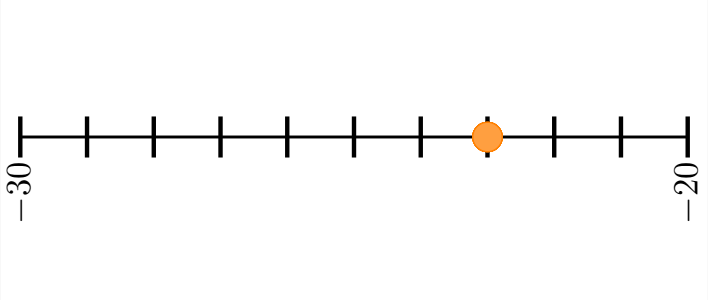
\includegraphics[width=0.8\linewidth]{../images/recta_num_-23.png}  \\[-1em]  \fillin[$-23$][1.5in]
                        \part 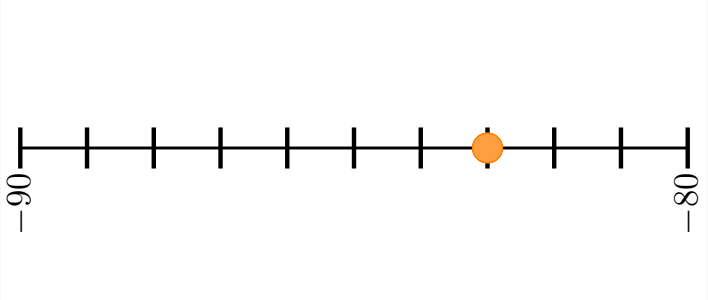
\includegraphics[width=0.8\linewidth]{../images/recta_num_-83.png}  \\[-1em]  \fillin[$-83$][1.5in]
                        \part 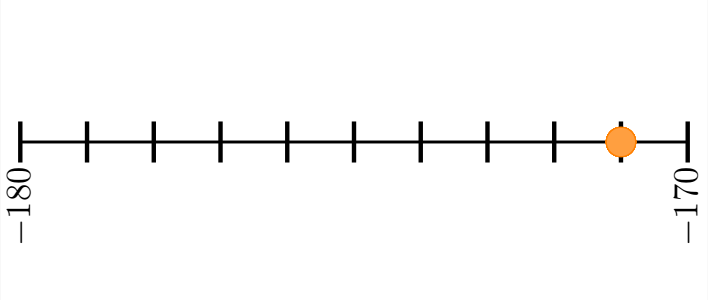
\includegraphics[width=0.8\linewidth]{../images/recta_num_-171.png} \\[-1em]   \fillin[$-171$][1.5in] 
		\end{parts}
	\end{multicols}
	}

      \questionboxed[4]{Escribe el número que representa el punto indicado en la recta numérica de cada uno de los siguientes incisos.

            \begin{multicols}{3}
                  \begin{parts}
                        \part 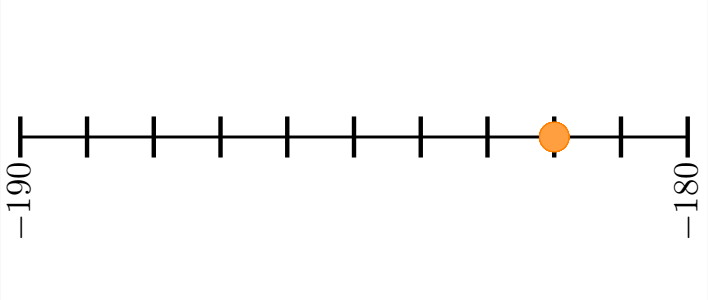
\includegraphics[width=0.8\linewidth]{../images/recta_num_-182.png} \\[-1em]   \fillin[$-182$][1.5in]
                        \part 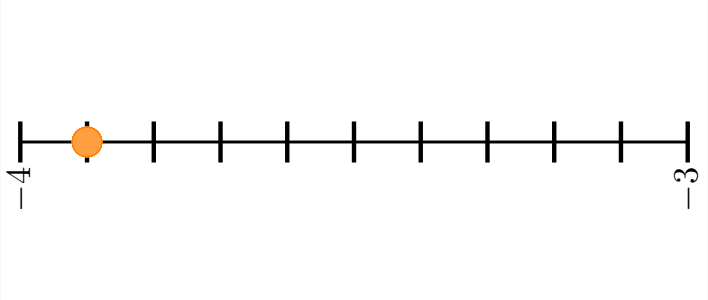
\includegraphics[width=0.8\linewidth]{../images/recta_num_-3.9.png} \\[-1em]  \fillin[$-3.9$][1.5in]
                        \part 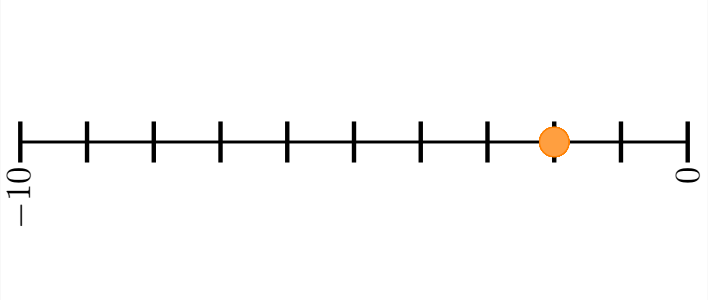
\includegraphics[width=0.8\linewidth]{../images/recta_num_-2.png}   \\[-1em]  \fillin[$-2$][1.5in]
                        \part 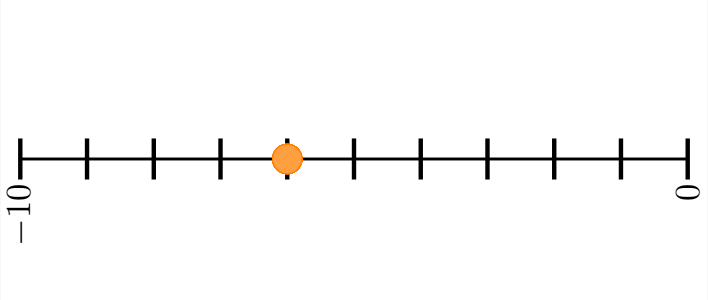
\includegraphics[width=0.8\linewidth]{../images/recta_num_-6.png}   \\[-1em]  \fillin[$-6$][1.5in]
                        \part 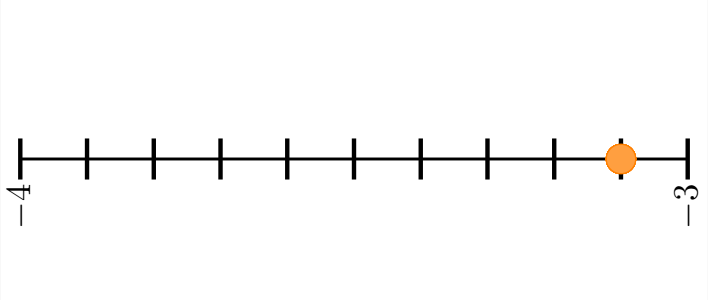
\includegraphics[width=0.8\linewidth]{../images/recta_num_-3.1.png} \\[-1em]   \fillin[$-3.1$][1.5in] 
                        \part 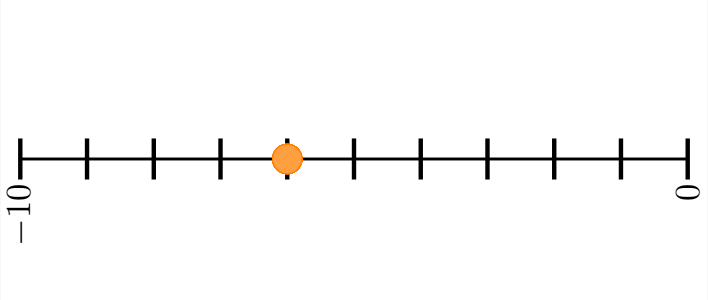
\includegraphics[width=0.8\linewidth]{../images/recta_num_-6.png}   \\[-1em] \fillin[$-6$][1.5in]     
                  \end{parts}
            \end{multicols}
      }

	  \ejemplosboxed[6]{Realiza las siguientes operaciones con números negativos:

	\begin{multicols}{3}
		\begin{parts}\normalsize
			\part $-223+67=$ \fillin[$-156$][0in]
			\part $(16)-(-14)=$ \fillin[$30$][0in]
			\part $(-16)+(-81)=$ \fillin[$-97$][0in]
		\end{parts}
	\end{multicols}
	}

      \questionboxed[8]{Realiza las siguientes operaciones de acuerdo con la jerarquía de operaciones:
           
      \begin{multicols}{3}
                  \begin{parts}\normalsize
                        \part $(64)-(-231)+(87)=$ \fillin[$382$][0in]
                        
						\part $(-16)+(-81)=$ \fillin[$-97$][0in]
                        
						\part $(121)-(54)+(-14)=$ \fillin[$53$][0in]
                        
						\part $(-13)-(91)=$ \fillin[$-104$][0in]
                        
						\part $(-97)+(55)=$ \fillin[$-42$][0in]
                        
						\part $(54)+(-97)+(-71)=$ \fillin[$-114$][0in]
                        
						\part $(57)+(-211)-(-81)=$ \fillin[$-73$][0in]
                        
						\part $(134)-(-94)=$ \fillin[$228$][0in]
                        
						\part $(16)-(-14)$ \fillin[$30$][0in]
                        
						\part $-23-(-67)$ \fillin[$44$][0in]
                        
						\part $-74-(-67)$ \fillin[$-7$][0in]
                        
						\part $-44-(-80)$ \fillin[$36$][0in]
                  \end{parts}
            \end{multicols}
      }

      \subsubsection{Comparación de negativos}
   
	  \ejemplosboxed[4]{Escribe sobre la línea el símbolo de mayor que ($>$), menor que ($<$), o igual ($=$) según corresponda.

	\begin{multicols}{2}
		\begin{parts}\normalsize
			\part $-182$ \fillin[$>$][0.5in] $-189$
			\part $-97$ \fillin[$<$][0.5in] $-96.2$
			\part $-51$ \fillin[$>$][0.5in] $-55$\\[0.1em]

		\end{parts}
	\end{multicols}
	}

      \questionboxed[4]{Escribe sobre la línea el símbolo de mayor que ($>$), menor que ($<$), o igual ($=$) según corresponda.
      
      \begin{multicols}{3}
                  \begin{parts}
                        \part $-59$ \fillin[$<$][0.5in] $-55$\\[0.1em]
                        % \part $-77$ \fillin[$>$][0.5in] $-177$\\[0.1em]
                        \part $-100$ \fillin[$<$][0.5in] $-99$\\[0.1em]
                        \part $-192$ \fillin[$<$][0.5in] $-189$\\[0.1em]
                        \part $-97$ \fillin[$<$][0.5in] $-96$\\[0.1em]
                        \part $-36$ \fillin[$>$][0.5in] $-39$\\[0.1em]
                        % \part $-3.5$ \fillin[$<$][0.5in] $-2.2$\\[0.1em]
                        \part $-12$ \fillin[$<$][0.5in] $-11$\\[0.1em]
                        % \part $-10.001$ \fillin[$>$][0.5in] $-100.01$\\[0.1em]
                        % \part $-0.99$ \fillin[$>$][0.5in] $1.01$\\[0.1em]
                        % \part $-3.9$ \fillin[$>$][0.5in] $-4.1$\\[0.1em]
                        % \part $-0.5$ \fillin[$<$][0.5in] $-0.4$\\[0.1em]
                        % \part $-1.2$ \fillin[$<$][0.5in] $-1.02$\\[0.1em]
                        % \part $-0.5$ \fillin[$>$][0.5in] $-0.6$\\[0.1em]
                  \end{parts}
            \end{multicols}
      }